%% Final edits by Jussi Kangasharju and Pirjo Moen
%% This file is modified by Veli Mäkinen from HY_fysiikka_LuKtemplate.tex authored by Roope Halonen ja Tomi Vainio.
%% Some text is also inherited from engl_malli.tex by Kutvonen, Erkiö, Mäkelä, Verkamo, Kurhila, and Nykänen.


% STEP 1: Choose oneside or twoside
\documentclass[english,twoside,openright]{UH_DS_MSc}
%finnish,swedish

%\usepackage[utf8]{inputenc} % For UTF8 support. Use UTF8 when saving your file.
\usepackage{lmodern} % Font package
\usepackage{textcomp} % Package for special symbols
\usepackage[pdftex]{color, graphicx} % For pdf output and jpg/png graphics
\usepackage[pdftex, plainpages=false]{hyperref} % For hyperlinks and pdf metadata
\usepackage{fancyhdr} % For nicer page headers
\usepackage{tikz} % For making vector graphics (hard to learn but powerful)
\usetikzlibrary{arrows.meta, positioning, automata, shapes.geometric, calc, fit, backgrounds}
%\usepackage{wrapfig} % For nice text-wrapping figures (use at own discretion)
\usepackage{amsmath, amssymb} % For better math
%\usepackage[square]{natbib} % For bibliography
\usepackage[footnotesize,bf]{caption} % For more control over figure captions
\usepackage{blindtext}
\usepackage{titlesec}
\usepackage[titletoc]{appendix}

\onehalfspacing %line spacing
%\singlespacing
%\doublespacing

%\fussy 
\sloppy % sloppy and fussy commands can be used to avoid overlong text lines

% STEP 2:
% Set up all the information for the title page and the abstract form.
% Replace parameters with your information.
\title{Performance, Safety, and Engineering Trade-offs of Rust and C++ in Nokia RAN Control-Plane Systems}
\author{Ha Vien}
\date{\today}
\prof{Christoph Luneburg, Petteri Kotimaa}
\censors{}{}{}
\keywords{Rust, C++, RAN control plane, tail latency, memory safety, fault injection, FFI}
\depositeplace{Helsinki University Library}
\additionalinformation{Software study track}


\classification{\protect{\ \\
\  Software and its engineering $\rightarrow$ Software notations and tools $\rightarrow$ General programming languages\  \\
\  Computer systems organization $\rightarrow$ Real-time systems $\rightarrow$ Real-time system specification\\
\  Networks $\rightarrow$ Network types $\rightarrow$ Mobile networks\\
}}

% if you want to quote someone special. You can comment this line and there will be nothing on the document.
%\quoting{Bachelor's degrees make pretty good placemats if you get them laminated.}{Jeph Jacques} 


% OPTIONAL STEP: Set up properties and metadata for the pdf file that pdfLaTeX makes.
% But you don't really need to do this unless you want to.
\hypersetup{
    %bookmarks=true,         % show bookmarks bar first?
    unicode=true,           % to show non-Latin characters in Acrobat’s bookmarks
    pdftoolbar=true,        % show Acrobat’s toolbar?
    pdfmenubar=true,        % show Acrobat’s menu?
    pdffitwindow=false,     % window fit to page when opened
    pdfstartview={FitH},    % fits the width of the page to the window
    pdftitle={Performance, Safety, and Engineering Trade-offs of Rust and C++ in Nokia RAN Control-Plane Systems},
    pdfauthor={Ha Vien},
    pdfsubject={Master's thesis, Computer Science},
    pdfcreator={Ha Vien},
    pdfproducer={pdfLaTeX}, % producer of the document
    pdfkeywords={Rust} {C++} {RAN control plane} {tail latency} {memory safety},
    pdfnewwindow=true,      % links in new window
    colorlinks=true,        % false: boxed links; true: colored links
    linkcolor=black,        % color of internal links
    citecolor=black,        % color of links to bibliography
    filecolor=magenta,      % color of file links
    urlcolor=cyan           % color of external links
}

\begin{document}

% Generate title page.
\maketitle

% STEP 3:
% Write your abstract (of course you really do this last).
% You can make several abstract pages (if you want it in different languages),
% but you should also then redefine some of the above parameters in the proper
% language as well, in between the abstract definitions.

\begin{abstract}
\noindent\textbf{Context.}
Radio Access Network (RAN) control-plane software (e.g.\ the L3 of a gNB) is written
mostly in C++ for performance, but C++ carries well-known memory-safety and concurrency
risks. Rust offers comparable performance with safety guaranteed at compile time, yet its
fit for latency-critical telecom control planes is unproven. The work is done at Nokia on
a subsystem modeled on a real Nokia gNB-CU-CP component.

\noindent\textbf{Objective.}
The thesis compares modern C++ and Rust on a UE Context Management service. As similar
average throughput is already known, it targets four less-explored dimensions: tail
latency and jitter under overload; which C++ defect classes Rust prevents at compile time;
the overhead of Rust's safety model; and the cost of incremental adoption in a C++ codebase.

\noindent\textbf{Methods.}
A language-agnostic specification is frozen first; two functionally equivalent
implementations are then built in C++ and Rust with identical algorithms, concurrency
model, allocator, and build settings. A synthetic, spec-justified workload is swept to
overload, both versions pass the same parity tests, and evaluation adds a fault-injection
study and a small FFI interoperability prototype.

\noindent\textbf{Results.}
Safety and migration results are final. Every one of five injected C++ defect classes
(use-after-free, double-free, iterator invalidation, data race, unguarded shared mutation) is
prevented at compile time in safe Rust, while in C++ each compiles and is caught, if at all,
only at runtime and only under the right sanitiser. The FFI migration prototype shows a small
seam that keeps the Rust core free of \texttt{unsafe} and adds no measurable per-call cost.
Preliminary performance measurements show the two languages tracking each other closely up to
saturation, with differences confined to the far tail; testbed-grade latency figures are the
remaining step.

\noindent\textbf{Conclusions.}
The thesis delivers a reproducible benchmarking framework, a parity-tested pair of
implementations, a defect-class taxonomy, and a quantified migration cost, and it argues that
for this class of subsystem the barrier to adopting Rust is engineering effort and the learning
curve rather than run-time performance.
\end{abstract}

% Place ToC
\mytableofcontents

\mynomenclature

% -----------------------------------------------------------------------------------
% STEP 4: Write the thesis.
% Your actual text starts here. You shouldn't mess with the code above the line except
% to change the parameters. Removing the abstract and ToC commands will mess up stuff.
\chapter{Introduction}

The mobile network is undergoing a profound softwarization. Functions that were once
delivered by fixed-function, vertically integrated hardware are being re-implemented as
software running on commodity servers, and the Radio Access Network (RAN), long the most
specialised part of the system, is no longer an exception. In the 5G NG-RAN architecture the
base station (gNB) is disaggregated into a central unit and one or more distributed units,
and the central unit is split again into control- and user-plane
functions~\cite{3gpp38401,3gpp38300}. Open-RAN initiatives push this disaggregation further,
turning the RAN into virtualised, multi-vendor software connected by open
interfaces~\cite{polese2023oran}. The resulting control plane, the gNB-CU-CP, is a large,
stateful, highly concurrent software system: it manages the lifecycle of every connected
device, drives the RRC signaling procedures~\cite{3gpp38331}, and coordinates mobility and
handovers, all under strict latency budgets and at very high event rates: a single busy site can drive on
the order of thousands of connection-management and mobility procedures per second, each
bounded by a budget measured in milliseconds~\cite{3gpp22261}, and a deployed control plane coordinates
millions of simultaneously connected devices. As the RAN moves to cloud-native,
disaggregated deployments, the correctness, reliability, and timing behaviour of this
software increasingly determine the quality of the network as a whole. An outage or a
tail-latency regression here is not a localised defect; it is a degradation felt across every
device the site serves~\cite{dean2013tail,barroso2017microseconds}.

This control-plane software is, today, written predominantly in C++. The choice is a
rational one: C++ offers the low-level control, mature tooling, and performance that
latency-critical systems demand. But that performance comes with a well-known cost. C++
places the burden of memory and concurrency management on the programmer, and decades of
experience show that this burden is routinely mishandled, producing use-after-free errors,
double-frees, data races, and related defects that are expensive to find, dangerous in
production, and responsible for a large share of security vulnerabilities in industry
practice~\cite{msrc2019memory,google2022android}. Rust has emerged as the first mainstream
systems language to promise an escape from this trade-off: memory safety and data-race
freedom enforced at compile time, with performance intended to be competitive with
C++~\cite{klabnik2023rust,jung2018rustbelt}. Whether that promise holds for a
telecom-grade, latency-critical control plane, where predictability under overload matters
as much as raw speed, is not well understood. This thesis, carried out at Nokia, addresses
the question directly: it develops two functionally equivalent implementations of a
representative RAN subsystem, a UE Context Management service modeled on a real Nokia
gNB-CU-CP component, in modern C++ and in Rust, and compares them under a realistic
synthetic signaling workload.

\section{Key terms and abbreviations}
For readers outside the telecom domain, Table~\ref{tab:abbrev} fixes the abbreviations and terms
used throughout the thesis. Three of them recur constantly: the \emph{gNB-CU-CP} is the
control-plane software this work is about; \emph{UE Context Management (UECM)} is the specific
subsystem reimplemented and measured; and \emph{tail latency} (the p99/p99.9 percentiles rather
than the mean) is the property that, more than average speed, decides whether such a system
meets its deadlines~\cite{dean2013tail,barroso2017microseconds}.

\begin{table}
\centering
\caption{Abbreviations and key terms used throughout the thesis.\label{tab:abbrev}}
\renewcommand{\arraystretch}{1.2}
\begin{tabular}{@{}p{0.17\linewidth} p{0.75\linewidth}@{}}
\hline\hline
Term & Meaning \\
\hline
RAN & Radio Access Network; the part of the mobile network connecting devices to the core \\
NG-RAN & Next-Generation RAN, the 5G radio-access-network architecture \\
gNB & 5G base station (``next-generation NodeB'') \\
gNB-CU / DU & Central Unit / Distributed Unit; the disaggregated halves of a gNB \\
gNB-CU-CP & Control-plane part of the central unit; the system class studied here \\
UE & User Equipment; an end device (phone, modem) attached to the network \\
UECM & UE Context Management; the per-UE state-management subsystem reimplemented here \\
RRC & Radio Resource Control; the control-plane signaling protocol between UE and gNB \\
DRB & Data Radio Bearer; a per-UE user-plane data channel set up during a session \\
Control plane & The signaling and management path, as opposed to the user-plane data path \\
Tail latency & High-percentile latency (p99, p99.9), the worst-case-oriented timing metric \\
FFI & Foreign Function Interface; calling Rust from C++ across a C ABI \\
HDR histogram & High-Dynamic-Range histogram, used for accurate latency capture \\
\hline
\end{tabular}
\end{table}

\section{Motivation and industrial context}
Two trends make this comparison timely. The first is the cloud-native evolution of the RAN
itself. Moving control-plane functions onto general-purpose servers raises, rather than
lowers, the premium on software quality: the software is longer-lived, evolves continuously,
runs at higher concurrency, and must meet its deadlines without the determinism that
purpose-built hardware once provided. This shift is accelerated by Open-RAN disaggregation,
which turns the base station into virtualised, multi-vendor software connected by open
interfaces~\cite{polese2023oran}, so that the control plane a vendor ships increasingly
competes on software-engineering quality rather than on bespoke hardware. In this setting a
latency regression or a memory-corruption defect is not a localised bug but a network-wide
reliability and security risk. The second trend is an industry-wide shift toward memory-safe languages. Large
software organisations report that the majority of their serious security vulnerabilities
stem from memory-safety errors, and that adopting memory-safe languages measurably reduces
them~\cite{msrc2019memory,google2022android,google2024securebydesign}. This concern has risen to the level of national
policy: cybersecurity agencies now urge software manufacturers to publish ``memory-safe
roadmaps'' and to migrate away from memory-unsafe languages such as C and
C++~\cite{cisa2023memorysafe,oncd2024building}. Rust in particular has moved from a niche
language into operating-system kernels, cloud infrastructure, and increasingly into
telecommunications; production hypervisors such as AWS Firecracker, which underpins its
serverless platform, are already written in Rust~\cite{agache2020firecracker}. Yet the evidence base for Rust's suitability rests largely on
general-purpose software and on average-case performance benchmarks. The specific question a
telecom vendor must answer, whether Rust can meet the tail-latency and predictability
requirements of a RAN control plane, whether it genuinely prevents the defect classes that
plague the existing C++ code, and what it costs to adopt it incrementally inside a large C++
codebase, has not been answered with direct, controlled evidence. Providing such evidence
for a representative subsystem is the motivation for this work.

\paragraph{Industrial setting.}
This thesis is carried out at Nokia, one of the small number of vendors that build, maintain,
and evolve production RAN software end to end, and the subsystem it studies, UE Context
Management (UECM), is modeled on a real gNB-CU-CP control-plane component rather than a
textbook example. The gNB-CU-CP is not a peripheral module: in the 3GPP disaggregated
architecture it is the control-plane half of the central unit, hosting RRC and managing the
UE context lifecycle while delegating user-plane bearer handling to the CU-UP over the E1
interface~\cite{3gpp38401,3gpp38300,3gpp38463,3gpp38331}, all under the millisecond-scale
procedure budgets the 5G system places on control signalling~\cite{3gpp22261}. Software of
this class is shipped, evolved, and operated across live operator networks, so a
language-selection decision here is a concrete production concern rather than a hypothetical
one, which is what makes a controlled comparison on a representative subsystem valuable to a
vendor. UECM is a deliberate choice of study object within that setting: it is small enough to
reimplement faithfully and to reason about in full, yet it exercises exactly the properties
that make RAN control-plane code hard: per-UE mutable state, a strict operation lifecycle,
high concurrency across many UEs, and hard tail-latency expectations. Conclusions drawn from
it therefore transfer to the broader class of stateful, concurrent control-plane services,
while remaining reproducible by readers outside Nokia because the implementation is driven
entirely by a public, frozen specification rather than by proprietary code.

\paragraph{A concrete failure mode.}
To make the stakes concrete, consider a mobility storm in which many UEs hand over at once. A
single mishandled pointer, a UE context freed on release while an in-flight signaling message
still references it, produces a use-after-free. In C++ this compiles cleanly and may pass
ordinary testing, only to corrupt an unrelated UE's state or crash the worker thread under
precisely the high-concurrency conditions the system exists to handle; the same latent race
can equally manifest as an unpredictable tail-latency spike rather than an outright crash. In
safe Rust the same design does not compile: ownership and borrowing reject the dangling
reference at build time. This one scenario captures why the thesis measures both
\emph{safety} (which defects are prevented, and when) and \emph{predictability} (tail
latency under overload) rather than average throughput alone.

\section{Nokia and the RAN control plane}
Nokia is one of the principal global suppliers of radio-access-network equipment and software,
competing to provide the gNB software that operators deploy at scale. The industry-wide
softwarization of the RAN---cloud-native deployment on commodity servers and Open-RAN's
disaggregation into virtualised, multi-vendor functions connected by open
interfaces~\cite{polese2023oran}---turns what was once embedded, hardware-bound functionality
into large, long-lived, continuously evolving software. For a vendor this reframes competitive
advantage around software qualities: reliability, predictable timing, security, and the pace at
which a large codebase can be evolved safely. It is in this context that a language-selection
question stops being academic and becomes a concrete engineering decision.

Within the gNB, the control-plane software (gNB-CU-CP) is among the most demanding parts of that
codebase. In the 3GPP architecture it hosts RRC and owns the UE-context lifecycle and mobility,
delegating user-plane bearers to the CU-UP over the E1
interface~\cite{3gpp38401,3gpp38300,3gpp38463,3gpp38331}, all under the millisecond-scale
procedure budgets the 5G system imposes~\cite{3gpp22261} and at the very high event rates and
connected-device counts a deployed network sustains. Because it is written in C++, it inherits
both that language's performance and its memory-safety and concurrency hazards. This is exactly
where the two pressures a RAN vendor now faces converge: the regulatory and security momentum
toward memory-safe languages~\cite{cisa2023memorysafe,oncd2024building,msrc2019memory}, and the
operational reality that tail latency under overload, rather than average throughput, governs
service quality~\cite{dean2013tail}. The UE Context Management subsystem studied in this thesis
is a faithful, self-contained proxy for that control-plane code, which is what lets a controlled
C++/Rust comparison on it speak directly to a decision a vendor such as Nokia must actually make,
while remaining reproducible outside the company because it is driven by a public specification
rather than by proprietary code.

\section{Challenges in RAN control-plane software engineering}
Modern RAN control-plane systems must be fast, predictable, highly concurrent, and
long-lived, and they are overwhelmingly written in C++. Two properties of this domain make
the language choice consequential. First, manual memory and concurrency management in C++
exposes the software to defects such as use-after-free, double-free, data races, and
iterator invalidation, which are silent at compile time and costly to find and fix at
telecom scale. Second, what governs whether RAN deadlines are met is not average throughput
but worst-case and tail behaviour under load and overload, a property that is easy to
regress and hard to measure correctly. Rust promises to remove the first class of defect at
compile time while claiming performance competitive on the second, but that claim rests
mostly on general-purpose benchmarks rather than on stateful, concurrent, latency-critical
telecom workloads. The next section turns these domain challenges into the specific,
unanswered questions this thesis sets out to address.

\section{Problem statement}
Bringing these threads together, the concrete problem this thesis addresses is the following.
Telecom vendors are under growing pressure, both technical and increasingly regulatory, to adopt
memory-safe languages, yet for the RAN control plane they lack \emph{direct, controlled}
evidence on which to base that decision. It is not established whether a Rust implementation of
a stateful, concurrent control-plane subsystem can match modern C++ in \emph{tail latency and
predictability under overload} (as opposed to average throughput), whether Rust's compile-time
guarantees actually eliminate the specific defect classes that afflict the existing C++ code,
and what incremental adoption \emph{costs} inside a large C++ codebase. The available evidence
is largely general-purpose and average-case~\cite{balasubramanian2017rust,qin2020rust}, leaving
these three questions (predictability, prevented-defect scope, and migration cost) open for a
representative subsystem. Answering them under controlled, reproducible conditions is the
problem this thesis sets out to solve.

\section{Research questions}
The thesis is organised around four research questions, ordered to put predictability and
migration ahead of raw average performance:

\begin{description}
  \item[RQ1] How do Rust and modern C++ compare in latency predictability (mean, p99,
        p99.9 tail latency, and jitter) for a RAN control-plane workload under increasing
        load and overload?
  \item[RQ2] Which classes of memory-safety and concurrency defects that occur in C++ are
        eliminated at compile time in the Rust implementation, and at what stage and cost
        are the remaining ones detected?
  \item[RQ3] What is the overhead, if any, of Rust's safety model (bounds checks,
        ownership-driven copies, abstraction cost) on throughput, CPU utilisation, and
        memory behaviour?
  \item[RQ4] What are the practical implications (effort, FFI interoperability, and risk)
        of adopting Rust incrementally within an existing C++ RAN software ecosystem?
\end{description}

\section{Research approach at a glance}
The four questions are answered constructively rather than by literature synthesis. The core
artifact is a pair of functionally equivalent UECM implementations, one in modern C++ and one in
Rust, built from a single frozen specification, so that any measured difference is attributable
to the language and its idioms rather than to divergent designs. RQ1 and RQ3 are answered by
driving both implementations with an identical, deterministic synthetic signaling workload in a
load sweep from light load through saturation, capturing latency with matched high-dynamic-range
histograms and resource use through the operating system, and comparing them with nonparametric
confidence intervals~\cite{georges2007rigorous}. RQ2 is answered by controlled fault injection:
a catalogue of representative C++ defects is written deliberately and each is confronted with its
Rust counterpart to record whether it is rejected at compile time, caught only at runtime, or
missed entirely. RQ4 is answered by building a working C++-to-Rust FFI prototype and measuring
the size of the interoperability seam, the scope of \texttt{unsafe}, and the per-call crossing
cost. The full protocol (testbed, workloads, and statistical treatment) is given in
Chapter~\ref{chapter:methodology}.

\section{Contributions, results, and limitations}
The thesis contributes (i) a reproducible, telecom-relevant benchmarking framework for
control-plane workloads; (ii) a frozen shared specification and two parity-tested
implementations of a RAN control-plane subsystem in C++ and Rust; (iii) a quantitative
comparison emphasising tail latency and predictability alongside average throughput;
(iv) a defect-class taxonomy obtained through controlled fault injection; and (v)
evidence-based engineering and migration guidelines for language selection in cloud-native
RAN evolution. The headline findings are as follows. On \emph{safety} (RQ2), every one of the
injected C++ defect classes is prevented at compile time in safe Rust, whereas in C++ each
compiles and is caught, if at all, only at runtime and only with the right sanitiser; this
result is final. On \emph{migration} (RQ4), the FFI seam is small, keeps the core free of
\texttt{unsafe}, and adds no measurable per-call cost, a sub-nanosecond crossing against an
operation roughly five orders of magnitude larger, so the real adoption cost is API design,
not run-time overhead; this result is also final. On \emph{performance} (RQ1, RQ3), preliminary
measurements collected on a development environment show the two implementations tracking each
other closely up to saturation, with differences confined to the far tail where the memory
allocator matters as much as the language; these numbers are preliminary because tail-latency
claims require the bare-metal testbed described in Chapter~\ref{chapter:methodology}. The main
limitations are the use of a synthetic workload, a single simplified subsystem, and
single-author implementation bias; these are treated in detail in
Chapter~\ref{chapter:discussion}.

\section{Significance and beneficiaries}
The results are intended to be directly actionable. For RAN vendors and cloud-native network
operators, the thesis supplies controlled evidence on the question that gates any language
decision. That question is not ``is Rust fast on average?'' but ``does Rust hold its tail latency and
predictability under overload, and what does incremental adoption cost?'', answered for a subsystem
representative of production control-plane code. For the standards and policy discussion around
memory-safe roadmaps~\cite{cisa2023memorysafe,oncd2024building}, it grounds a general mandate in
a concrete telecom data point. For the research community, the frozen specification, the
parity-tested implementations, the reproducible benchmarking framework, and the defect-class
taxonomy form a reusable baseline for further language and systems studies. And for practising
engineers, the fault catalogue and the migration prototype double as worked examples of what
Rust's guarantees do and do not buy in this domain.

\section{Thesis outline}
Chapter~\ref{chapter:background} gives the background on RAN control-plane software, C++,
and the Rust safety model. Chapter~\ref{chapter:methodology} states the research approach.
Chapter~\ref{chapter:context} describes the problem context: the UE Context Management
subsystem, the relevant defect classes, and tail-latency predictability.
Chapter~\ref{chapter:objectives} sets the objectives, scope, and boundaries.
Chapter~\ref{chapter:design} presents the design and implementation of both versions.
Chapter~\ref{chapter:eval} describes the experimental setup and reports the evaluation.
Chapter~\ref{chapter:discussion} discusses the findings, related work, and threats to
validity. Chapter~\ref{chapter:conclusions} concludes and outlines future work.
Figure~\ref{fig:roadmap} summarises this structure at a glance.

\begin{figure}
\centering
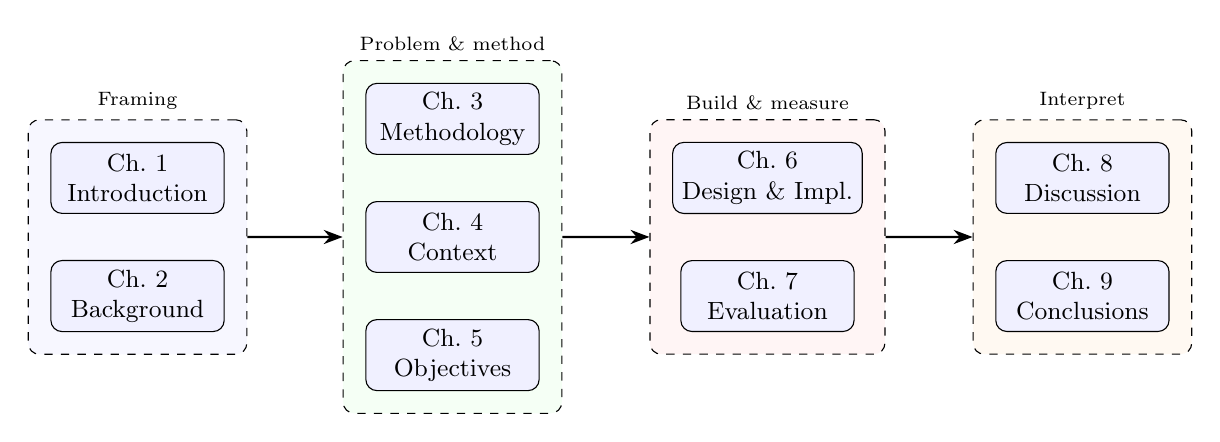
\begin{tikzpicture}[
    font=\small,
    stage/.style={draw, rounded corners, align=center, minimum width=2.2cm,
                  minimum height=0.9cm, fill=blue!6},
    grp/.style={draw, dashed, rounded corners, inner sep=8pt},
    >={Stealth[length=2.4mm]}
  ]
  \node[stage] (c1) at (0,0.75)  {Ch.~1\\ Introduction};
  \node[stage] (c2) at (0,-0.75) {Ch.~2\\ Background};

  \node[stage] (c3) at (4,1.5)   {Ch.~3\\ Methodology};
  \node[stage] (c4) at (4,0.0)   {Ch.~4\\ Context};
  \node[stage] (c5) at (4,-1.5)  {Ch.~5\\ Objectives};

  \node[stage] (c6) at (8,0.75)  {Ch.~6\\ Design \& Impl.};
  \node[stage] (c7) at (8,-0.75) {Ch.~7\\ Evaluation};

  \node[stage] (c8) at (12,0.75) {Ch.~8\\ Discussion};
  \node[stage] (c9) at (12,-0.75){Ch.~9\\ Conclusions};

  \begin{scope}[on background layer]
    \node[grp, fill=blue!3,   fit=(c1)(c2)]      (g1) {};
    \node[grp, fill=green!4,  fit=(c3)(c4)(c5)]  (g2) {};
    \node[grp, fill=red!4,    fit=(c6)(c7)]      (g3) {};
    \node[grp, fill=orange!5, fit=(c8)(c9)]      (g4) {};
  \end{scope}

  \node[font=\scriptsize, above] at (g1.north) {Framing};
  \node[font=\scriptsize, above] at (g2.north) {Problem \& method};
  \node[font=\scriptsize, above] at (g3.north) {Build \& measure};
  \node[font=\scriptsize, above] at (g4.north) {Interpret};

  \draw[->, thick] (g1.east) -- (g2.west);
  \draw[->, thick] (g2.east) -- (g3.west);
  \draw[->, thick] (g3.east) -- (g4.west);
\end{tikzpicture}
\caption{Roadmap of the thesis. The chapters progress from framing the problem, through the
research method and problem context, to the constructed artifacts and their evaluation, and
finally to interpretation and conclusions.\label{fig:roadmap}}
\end{figure}

\chapter{Background: Systems Languages for Latency-Critical Software\label{chapter:background}}

\section{RAN control-plane systems and the gNB-CU-CP}
The NG-RAN architecture splits the gNB into a central unit (gNB-CU) and distributed units,
with the control plane (gNB-CU-CP) handling RRC and connection management for each
UE~\cite{3gpp38401,3gpp38300,3gpp38331}. Such control-plane systems must satisfy demanding
non-functional requirements: very high event rates (UE mobility, signaling storms), strict
and predictable latency bounds that the 5G service specifications quantify as
KPIs~\cite{3gpp22261}, long-lived software with continuously evolving complexity,
and heavily concurrent workloads. In these systems the worst-case and tail behaviour,
rather than the average, determines whether deadlines are met, which motivates the
predictability focus of this thesis.

Functionally, the gNB is disaggregated along two orthogonal axes. The first is a
\emph{central/distributed} split: a central unit (gNB-CU) hosts the higher layers of the
protocol stack, while one or more distributed units (gNB-DU) host the lower, more
time-critical layers close to the radio. The second is a \emph{control/user-plane} split
inside the central unit, separating the control-plane function (gNB-CU-CP) from the
user-plane function (gNB-CU-UP). These parts communicate over standardised
interfaces---NG towards the 5G core, F1 between the CU and the DU, and E1 between the CU-CP and
the CU-UP~\cite{3gpp38401,3gpp38300,3gpp38463}. Open-RAN initiatives standardise these interfaces
further so that each part can be supplied by a different vendor and run as software on
commodity hardware~\cite{polese2023oran}. Figure~\ref{fig:ngran} places the subsystem studied
in this thesis, UE Context Management (UECM), inside the gNB-CU-CP: it owns the per-UE
control-plane state and mediates the RRC signaling and mobility procedures, which is why its
correctness and timing behaviour are representative of the control plane as a whole.

\begin{figure}
\centering
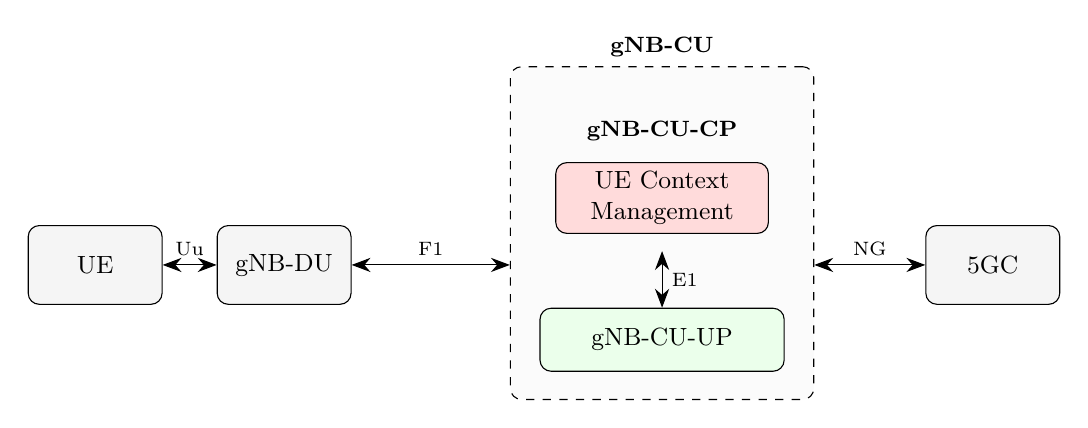
\begin{tikzpicture}[
    font=\small, >={Stealth[length=2.4mm]},
    box/.style={draw, rounded corners, minimum height=1.0cm, minimum width=1.7cm,
                align=center, fill=gray!8},
    cpbox/.style={draw, rounded corners, align=center, fill=blue!8},
    upbox/.style={draw, rounded corners, minimum width=3.1cm, minimum height=0.8cm,
                  align=center, fill=green!8},
    uecm/.style={draw, rounded corners, minimum width=2.7cm, minimum height=0.62cm,
                 fill=red!14, align=center}
  ]
  \node[box] (ue) at (0,0)   {UE};
  \node[box] (du) at (2.4,0) {gNB-DU};

  % Control plane, with UE Context Management shown nested inside it
  \node[font=\footnotesize\bfseries] (cpttl) at (7.2,1.7) {gNB-CU-CP};
  \node[uecm] (uecm) at (7.2,0.85) {UE Context\\ Management};
  \begin{scope}[on background layer]
    \node[cpbox, fit=(cpttl)(uecm), inner sep=6pt] (cp) {};
  \end{scope}
  % User plane
  \node[upbox] (up) at (7.2,-0.95) {gNB-CU-UP};

  \begin{scope}[on background layer]
    \node[draw, dashed, rounded corners, fill=gray!3,
          fit=(cp)(up), inner sep=10pt, label={[font=\footnotesize\bfseries]above:gNB-CU}] (cu) {};
  \end{scope}

  \node[box] (core) at (11.4,0) {5GC};

  \draw[<->] (ue) -- node[above,font=\scriptsize]{Uu} (du);
  \draw[<->] (du.east)         -- node[above,font=\scriptsize]{F1} (cu.west |- du);
  \draw[<->] (cu.east |- core) -- node[above,font=\scriptsize]{NG} (core.west);
  \draw[<->] (cp.south) -- node[right,font=\scriptsize]{E1} (up.north);
\end{tikzpicture}
\caption{Where the studied subsystem sits in the 5G NG-RAN. The gNB is split into a
distributed unit (gNB-DU) and a central unit (gNB-CU), and the central unit is split again
into control-plane (gNB-CU-CP) and user-plane (gNB-CU-UP) functions, connected by the
standardised F1, E1, and NG interfaces. UE Context Management (highlighted) is the per-UE
control-plane state manager inside the gNB-CU-CP that this thesis reimplements and
measures.\label{fig:ngran}}
\end{figure}

\section{Latency, throughput, and predictability in real-time software}
Latency-critical systems are judged less by how much work they do on average than by how
\emph{predictably} they do it. Three metrics must be distinguished. \emph{Throughput} is the
sustained rate of completed operations; \emph{latency} is the time an individual operation
takes; and \emph{jitter} is the variability of that latency. Because a system can have
excellent mean latency and still miss deadlines often, the meaningful figures are the
high-percentile \emph{tail} latencies---the 99th (p99) and 99.9th (p99.9) percentiles---rather
than the mean. At the scale of a network, tail latency dominates user-visible behaviour: when
a single user action fans out into many internal operations, the slowest of them sets the
response time, so rare per-operation delays become common per-request delays~\cite{dean2013tail}.
Modern data-centre and networking software increasingly operates in a regime where the
relevant latencies are measured in microseconds, a range in which conventional
operating-system and software overheads are no longer negligible~\cite{barroso2017microseconds}.
Fine-grained measurement studies show that, even at moderate utilisation, hardware, operating-system,
and application-level effects such as background interference, scheduling, interrupt routing, and
power-saving states inflate the tail far beyond what queueing models predict~\cite{li2014tales}.

\begin{figure}
\centering
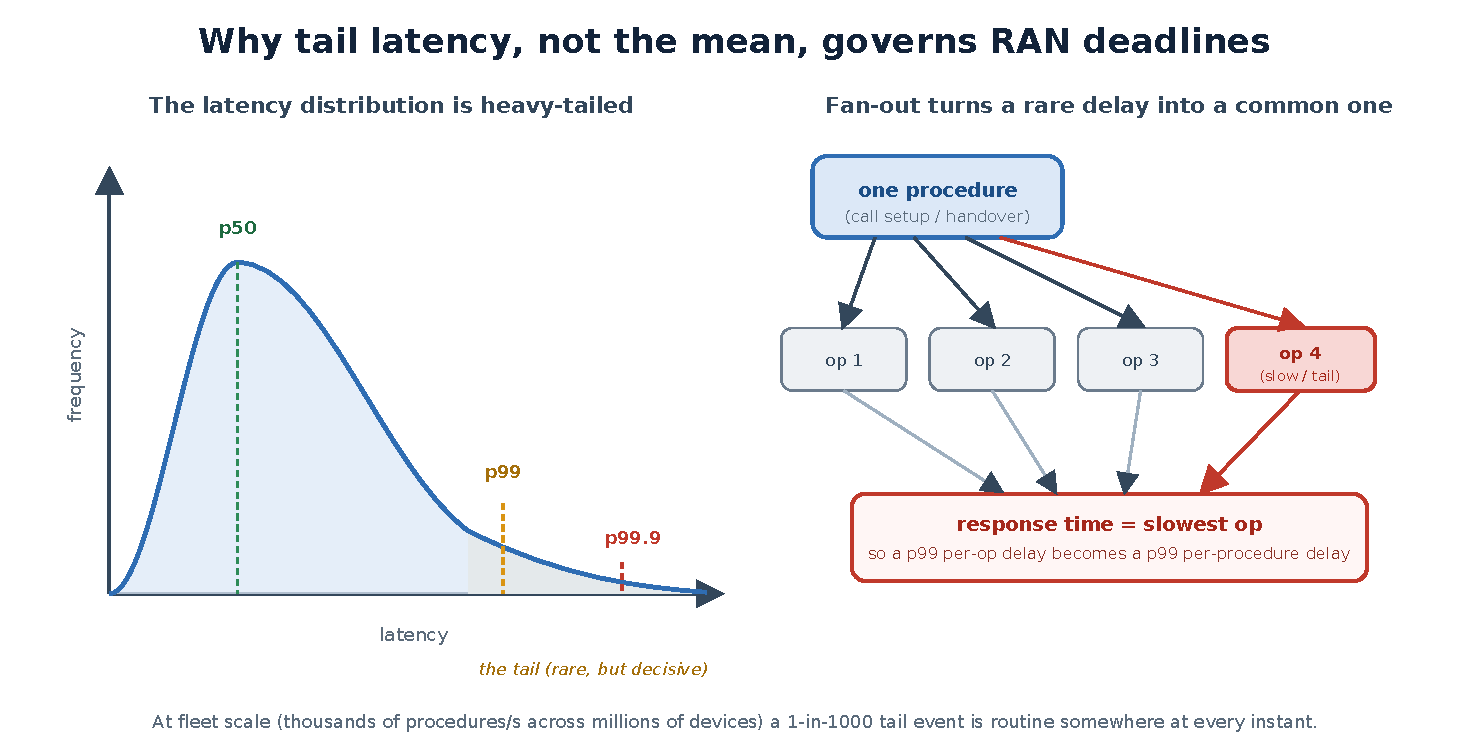
\includegraphics[width=\linewidth]{diagrams/pdf/11_tail_latency_concept.pdf}
\caption{Why the tail, not the mean, governs RAN deadlines. The latency distribution is
heavy-tailed (left), so the p99/p99.9 percentiles lie far from the median. Because a single
procedure fans out into many dependent operations whose slowest member gates completion (right),
a delay that is rare per operation becomes common per procedure; at fleet scale a one-in-a-thousand
tail event is routine somewhere at every instant.\label{fig:tailconcept}}
\end{figure}

Real-time systems are conventionally graded by the consequence of a missed deadline: in
\emph{hard} real-time a miss is a failure, in \emph{firm} real-time a late result is useless
but not catastrophic, and in \emph{soft} real-time a miss merely degrades quality. A RAN
control plane is best seen as soft-to-firm real-time: an occasional late signaling response
degrades service rather than endangering it, but at fleet scale and under signaling storms
such degradations accumulate into a network-wide reliability problem. This is compounded by
queueing behaviour: as offered load approaches service capacity, queueing delay grows
sharply and the latency tail explodes near saturation. Characterising a system therefore
requires driving it not just at nominal load but \emph{into overload}, which is why the
evaluation in this thesis sweeps load up to and beyond the saturation point.

Measuring tail latency correctly is itself a pitfall. A naive closed-loop load generator
that waits for each response before issuing the next request suffers \emph{coordinated
omission}: when the system stalls, the generator stalls with it and simply fails to record
the many requests that would have arrived during the stall, systematically hiding the very
tail it is meant to expose. Sound measurement therefore requires an open-loop model with an
intended schedule, correction for coordinated omission, high-dynamic-range latency histograms
that retain resolution across many orders of magnitude, and statistically rigorous reporting
with repeated runs and confidence intervals rather than single point
estimates~\cite{georges2007rigorous}. These techniques are applied in
Chapter~\ref{chapter:eval}.

\begin{figure}
\centering
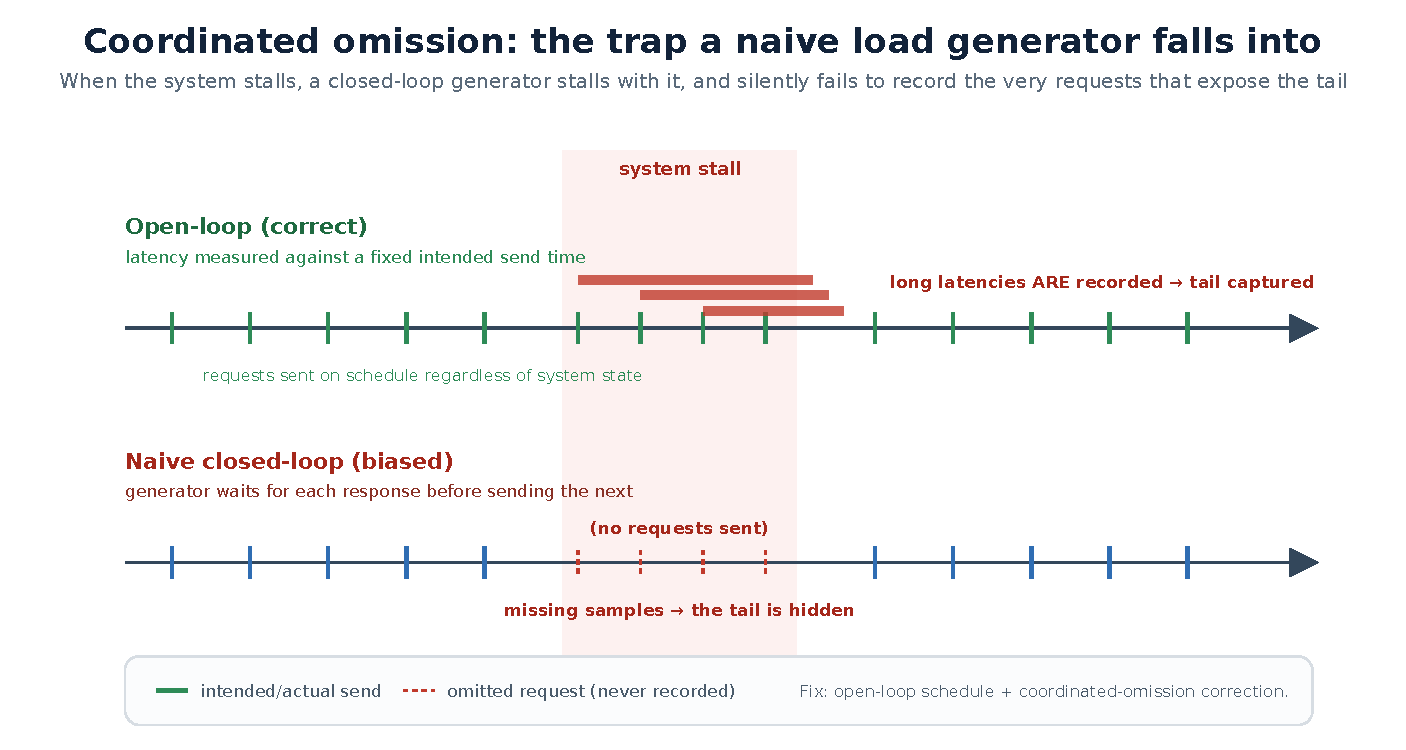
\includegraphics[width=\linewidth]{diagrams/pdf/16_coordinated_omission.pdf}
\caption{Coordinated omission. An open-loop generator (top) sends on a fixed intended schedule
regardless of system state, so requests issued during a stall are recorded with their full
latency and the tail is captured. A naive closed-loop generator (bottom) waits for each response
before sending the next, so when the system stalls it stalls too and never issues the delayed
requests---silently omitting exactly the samples that would expose the tail.\label{fig:coord}}
\end{figure}

\section{C++ for latency-critical systems}
C++ is the default language for RAN control-plane software for good reasons. It offers
zero-overhead abstractions, direct control over memory layout and allocation, deterministic
destruction through the Resource Acquisition Is Initialization (RAII) idiom, and mature
compilers, libraries, and profiling tools, all without a garbage collector that could inject
unpredictable pauses. Modern C++ (C++11 and later) adds smart pointers
(\texttt{std::unique\_ptr}, \texttt{std::shared\_ptr}) that automate ownership, move semantics
that avoid needless copies, and a formal memory model with \texttt{std::atomic} for
lock-based and lock-free concurrency. These features make it possible to write fast and, with
discipline, reasonably safe systems code.

The difficulty is that safety in C++ remains the programmer's responsibility rather than a
property the compiler enforces. RAII and smart pointers reduce but do not eliminate temporal
errors: raw pointers and references can outlive the objects they point to, iterators can be
invalidated by container mutation, objects can be used after a move, and nothing in the type
system prevents a mutable object from being aliased and mutated concurrently from several
threads. The result is a well-known catalogue of defects---use-after-free, double-free,
buffer overflow, data races, deadlocks, and iterator invalidation---that are easy to
introduce and expensive to find at telecom scale. Memory-corruption errors of this kind have
been a persistent security problem for decades, and deployed mitigations remain only partial
defences~\cite{szekeres2013sok}. Their prevalence is well documented in
industry: memory-safety issues account for roughly 70\,\% of the security vulnerabilities
reported at Microsoft~\cite{msrc2019memory}, and Google reports a sharp drop in such
vulnerabilities as memory-safe languages are adopted in Android~\cite{google2022android}. This
specific catalogue is developed in detail in Chapter~\ref{chapter:context} and forms the basis
for the fault-injection study in Chapter~\ref{chapter:eval}.

C++ practice mitigates these defects with tooling rather than with language guarantees, and
the tooling is inherently partial. Dynamic sanitizers such as AddressSanitizer (ASan),
ThreadSanitizer (TSan), and UndefinedBehaviorSanitizer detect many errors, but only on the
code paths that a given test actually executes with the right inputs, and they impose runtime
and memory overheads that make them unsuitable for production; TSan in particular reports only
those data races that happen to occur during a run, so a race that manifests only under a rare
interleaving can pass unnoticed. Static analysers help but suffer false negatives and cannot
reason about the whole program. Detection is therefore best-effort and after the fact, which
is precisely the situation a language with compile-time guarantees is meant to change.

\section{The Rust ownership and safety model}
Rust offers memory safety and data-race freedom enforced at compile time through its
ownership and borrowing model~\cite{klabnik2023rust}, together with a strong concurrency
story and modern tooling (Cargo, integrated testing). It is the first industry-supported
language to overcome the traditional trade-off between the safety of high-level languages and
the low-level control of C and C++, achieving this with a type system based on ownership and
borrowing that statically forbids the mutation of shared state, while confining the
unavoidable exceptions to \texttt{unsafe} code encapsulated behind safe
APIs~\cite{jung2021safe}. The soundness of the safe fragment of the language, including the
role of \texttt{unsafe} as an explicitly delimited escape hatch, has been established formally
by the RustBelt project~\cite{jung2018rustbelt}, and the aliasing discipline that even
\texttt{unsafe} code must respect has been given a precise operational
semantics~\cite{jung2020stacked}. Empirical evidence supports the model in
practice: \texttt{unsafe} is used sparingly and in localised ways in real
codebases~\cite{astrauskas2020unsafe,qin2020rust}, and a study of all Rust memory-safety CVEs
found that every one of them involved \texttt{unsafe} code, confirming that safe Rust keeps
its promise~\cite{xu2021rustcve}. The caveat is that unsafety propagates through dependencies:
although fewer than a third of libraries use \texttt{unsafe} directly, a much larger fraction
cannot be fully statically checked because \texttt{unsafe} hides somewhere in their call
chain~\cite{evans2020rust}, which is a further argument for keeping the safety-critical core of
a subsystem \texttt{unsafe}-free, as this thesis does. Crucially for a latency-critical setting, this safety is
enforced by the type system and borrow checker rather than by runtime instrumentation, and is
intended to be \emph{zero-cost}: systems research argues Rust attains safety without the
overhead of garbage collection or runtime checks, and even enables efficiency techniques that
are impractical in C~\cite{balasubramanian2017rust}. Whether that zero-cost claim holds for a
telecom control-plane workload is precisely the property this thesis evaluates.

Concretely, the borrow checker rejects at compile time the very use-after-free sketched in the
introduction. The following program does not build, because \texttt{ctx} is moved (dropped)
while a reference to it is still live:

\begin{verbatim}
    let ctx = UeContext::new(42);
    let r = &ctx;      // immutable borrow of ctx
    drop(ctx);         // move/free ctx ...
    use_ctx(r);        // error[E0505]: cannot move out of `ctx`
                       //              because it is borrowed
\end{verbatim}

\noindent The same discipline extends to concurrency. Rust encodes thread-safety in the type
system through the \texttt{Send} and \texttt{Sync} marker traits: a value may cross a thread
boundary only if its type is \texttt{Send}, and may be shared by reference across threads only
if it is \texttt{Sync}. Sharing a value that permits unsynchronised mutation is therefore a
compile error, not a latent race---the property Rust markets as ``fearless concurrency.''
Error handling is likewise explicit: fallible operations return a \texttt{Result} value that
the caller must handle, rather than raising an exception that unwinds through hidden control
flow, which keeps the cost and the control flow of the failure path visible---an advantage in
latency-sensitive code where surprises in the tail are what matter.

\begin{figure}
\centering
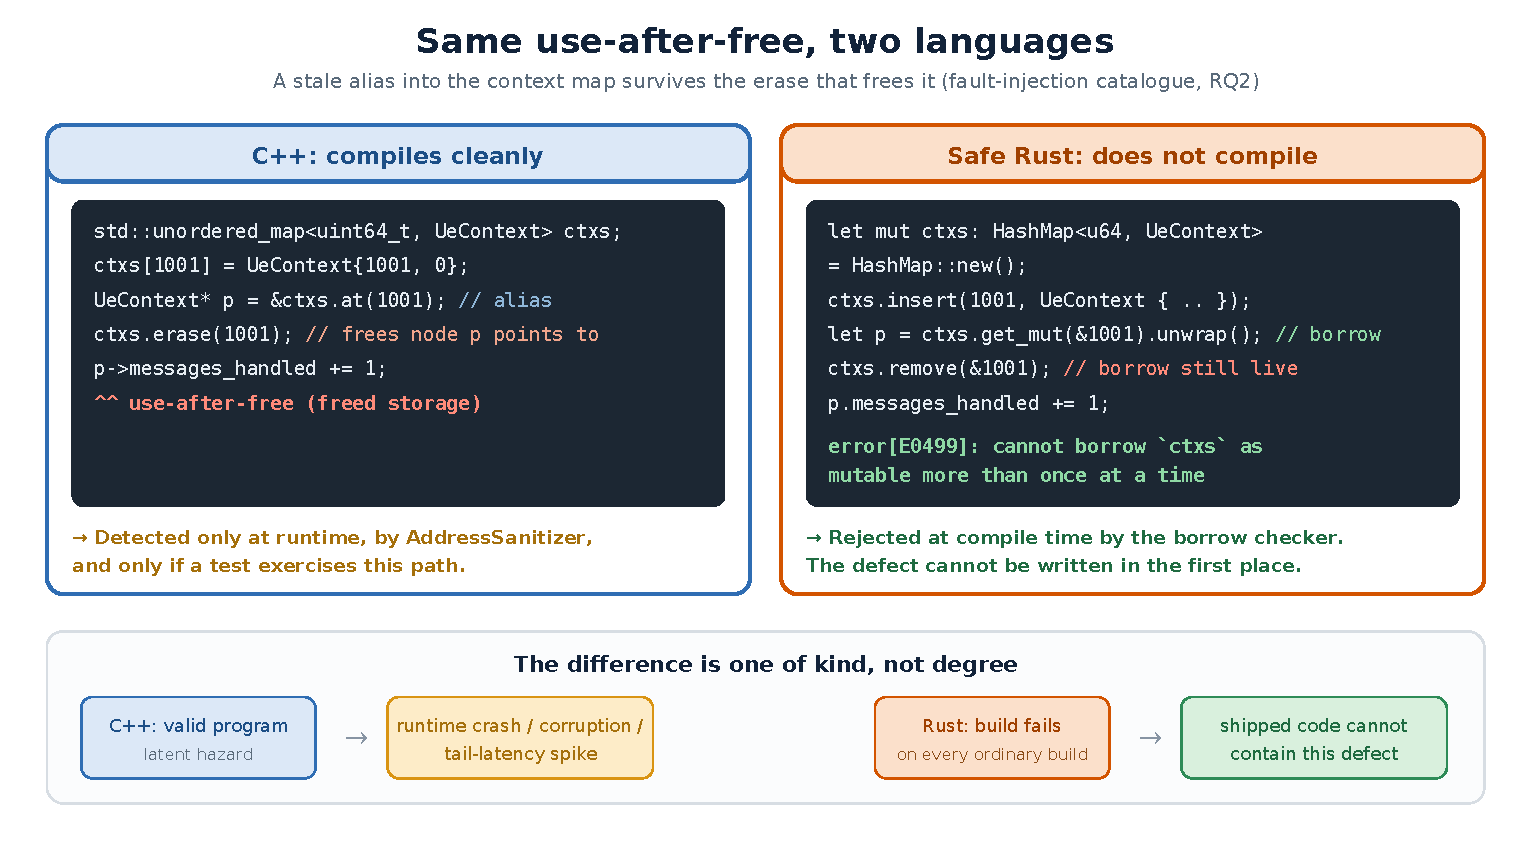
\includegraphics[width=\linewidth]{diagrams/pdf/08_borrow_checker_uaf.pdf}
\caption{The same use-after-free defect in C++ and in safe Rust. The stale alias into the
context map survives the \texttt{erase}/\texttt{remove} that frees it: in C++ this compiles and
is caught only at runtime (and only under AddressSanitizer, on a path a test exercises), whereas
in safe Rust the borrow checker rejects it at compile time (\texttt{E0499}), so the defect
cannot be written at all. The difference is one of kind, not degree.\label{fig:borrowuaf}}
\end{figure}

\section{The systems-language landscape}
Rust is not the only memory-safe language, but it occupies a distinctive position for this
problem. Managed languages such as Java, C\#, and Go achieve memory safety through a runtime
and garbage collection. That is an excellent trade for much software, but it is a poor fit for
a tail-latency-critical control plane: garbage collection introduces pauses and timing
variability that are a recognised source of tail latency in large systems~\cite{dean2013tail},
and a managed runtime also cedes the low-level control over memory layout and scheduling that
this domain relies on. At the other extreme, C is as memory-unsafe as C++ while offering fewer
abstractions for building large systems. Rust is the first widely supported language to
combine memory and thread safety, enforced at compile time, with the absence of a garbage
collector and performance intended to be competitive with C++~\cite{jung2021safe,
balasubramanian2017rust}; cross-language benchmark surveys place Rust's throughput and memory
use alongside C and C++ while it retains its safety guarantees~\cite{bugden2022rust}. That
combination is exactly why the meaningful comparison for RAN
control-plane software is C++ against Rust, and why managed languages are out of scope here.

\begin{figure}
\centering
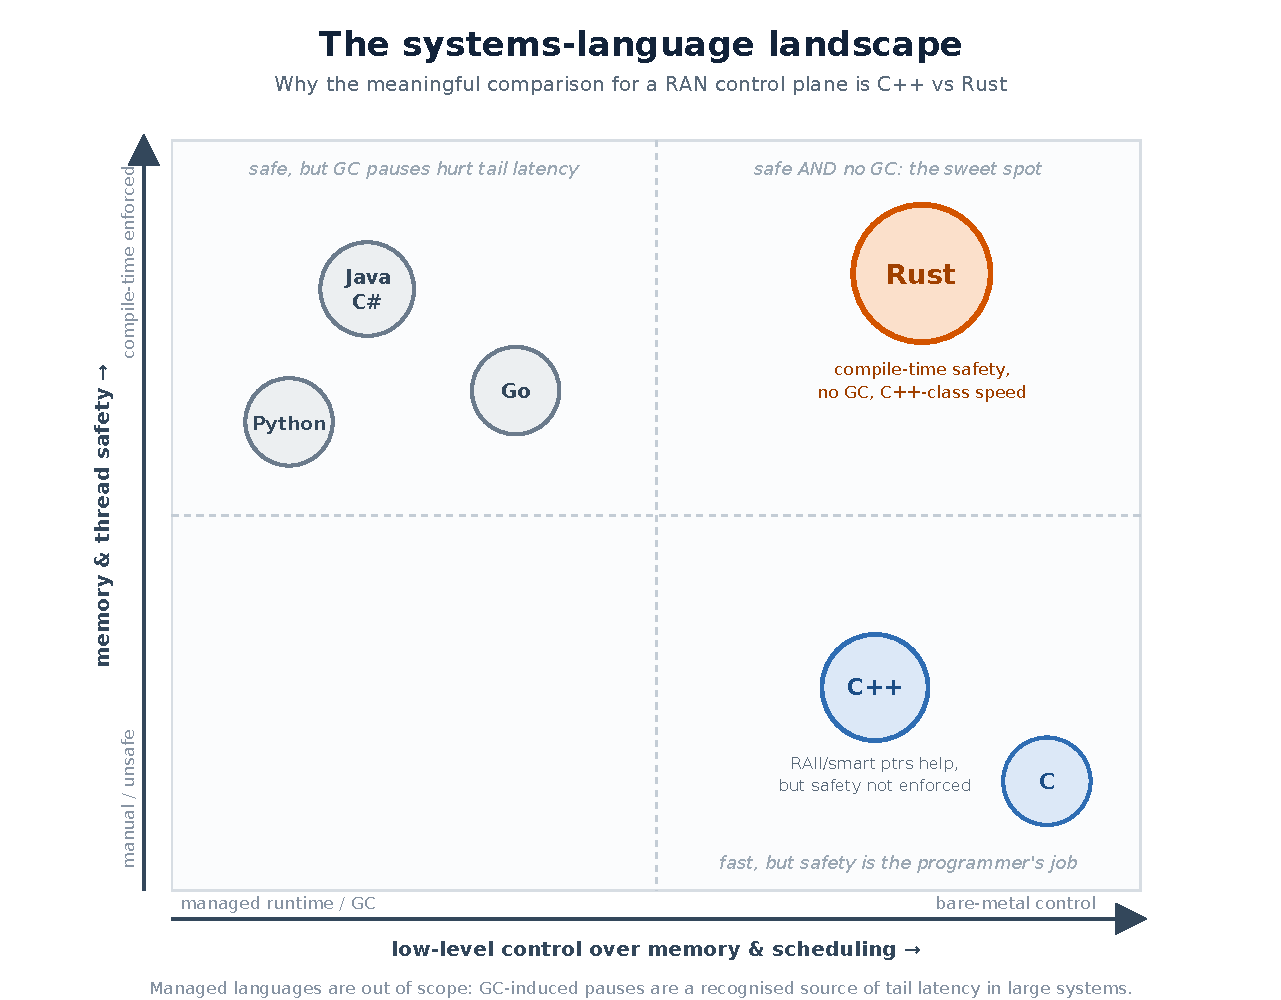
\includegraphics[width=0.82\linewidth]{diagrams/pdf/09_language_landscape.pdf}
\caption{The systems-language landscape along two axes: low-level control over memory and
scheduling (horizontal) and memory/thread safety (vertical). Managed languages (Java, C\#, Go,
Python) are safe but pay a garbage-collection cost that hurts tail latency; C and C++ give
bare-metal control but leave safety to the programmer. Rust occupies the sweet spot---compile-time
safety with no garbage collector---which is why the meaningful comparison for a RAN control plane
is C++ against Rust.\label{fig:landscape}}
\end{figure}

\section{Concurrency models for control-plane software}
How concurrency is structured shapes both correctness and tail latency. The dominant model is
\emph{shared-memory} concurrency, in which threads mutate common state guarded by mutexes and
atomics; it is flexible but is the source of races, deadlocks, lock contention, and priority
inversion, and its worst-case timing is hard to reason about. The alternative is
\emph{message-passing} or \emph{shared-nothing} concurrency, in which state is partitioned so
that each piece is owned by a single thread and all interaction happens through messages, as
in the actor model and in sharded designs. Shared-nothing trades some flexibility for
scalability and far simpler reasoning, and it maps naturally onto per-UE partitioning in a
control plane, where each UE's state is largely independent.

A second, orthogonal choice is how work is queued between producers and consumers. Unbounded
queues mask overload and let latency and memory grow without limit; \emph{bounded} queues with
either blocking (backpressure) or shedding bound worst-case memory and make overload visible,
which is essential for predictable tail latency. Lock-free structures can reduce contention
but are notoriously difficult to implement correctly. These considerations directly motivate
the architecture adopted for both implementations in Chapter~\ref{chapter:design}: a
shared-nothing, thread-per-shard design with bounded multi-producer/single-consumer queues and
blocking backpressure, chosen so that any measured latency difference reflects the language
rather than a divergent concurrency strategy.

\begin{figure}
\centering
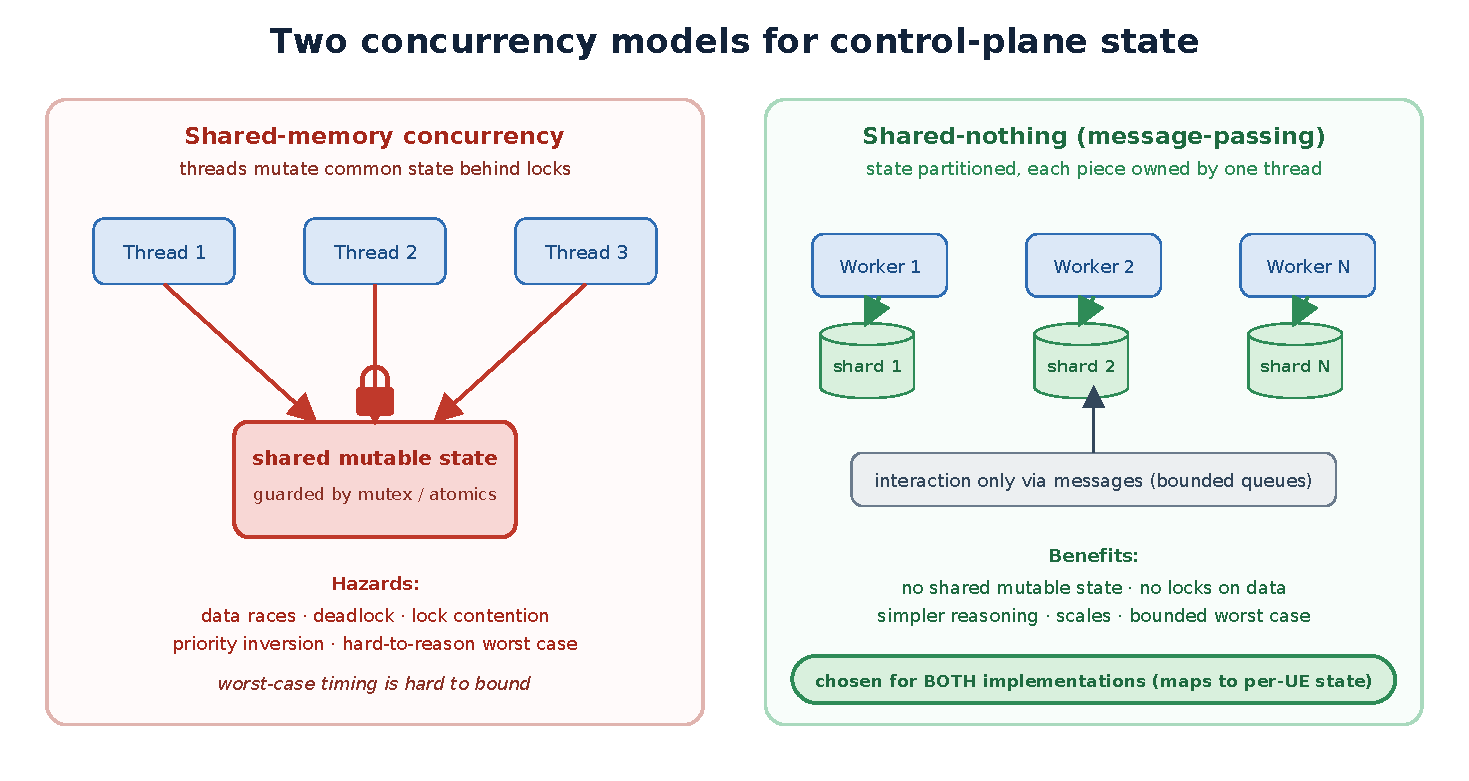
\includegraphics[width=\linewidth]{diagrams/pdf/12_concurrency_models.pdf}
\caption{Two concurrency models for control-plane state. Shared-memory concurrency (left) lets
threads mutate common state behind locks and is the source of data races, deadlock, and lock
contention, with a worst case that is hard to bound. Shared-nothing message-passing (right)
partitions state so each shard is owned by a single worker and all interaction happens through
bounded queues; this eliminates locks on context data and maps naturally onto per-UE
partitioning, and is the model adopted for both implementations.\label{fig:concmodels}}
\end{figure}

\section{Interoperability between C++ and Rust}
Adopting a new language in a large existing system is necessarily incremental: a Rust
component must coexist with, and be callable from, a substantial C++ codebase. The common
denominator for such interoperability is the C application binary interface (ABI). Rust can
expose functions with \texttt{extern "C"} linkage and hand out \emph{opaque handles} to
Rust-owned objects, which C++ then calls through a C header; tooling automates parts of this,
including \texttt{bindgen} (generating Rust bindings from C headers), \texttt{cbindgen}
(generating C headers from Rust), and the \texttt{cxx} crate (a safer bidirectional bridge).
Interoperability is not free: crossing the boundary steps outside the checked language, so the
seam must contain \texttt{unsafe} code; passing anything beyond simple values requires
marshalling; and the shape of the foreign interface has to be designed deliberately. The size
of that seam, how much \texttt{unsafe} it concentrates, and the per-call crossing cost are
exactly the quantities measured for RQ4 in Chapter~\ref{chapter:eval}.

\section{Research gap}
The preceding sections establish three things. First, the RAN control plane is a
soft-to-firm real-time, highly concurrent, latency-critical domain in which tail behaviour
under overload, not average throughput, governs the quality experienced by the network.
Second, C++ supplies the control and performance this domain demands but leaves whole classes
of memory and concurrency defects to best-effort, after-the-fact detection. Third, Rust
promises to prevent those classes at compile time at no runtime cost, with a credible
incremental adoption path through C-ABI interoperability. What is missing from the literature
is \emph{direct, controlled} evidence for a representative control-plane subsystem: whether
Rust actually holds its tail latency and predictability under overload against modern C++,
exactly which defect classes it eliminates and at what stage the remainder are caught, what
its safety model costs in throughput and resources, and what incremental adoption costs in
practice. Closing this gap is the purpose of the four research questions, pursued with the
methodology set out in Chapter~\ref{chapter:methodology}.

\chapter{Research Methodology\label{chapter:methodology}}

\section{Research approach}
The thesis follows an empirical, experimental research approach with a constructive
(design-science) element. A software artifact, two functionally equivalent implementations
of the subsystem together with a benchmarking framework, is built against a single frozen
specification and then evaluated under controlled experiments. Evidence is triangulated from
three complementary methods: quantitative performance measurement under a swept load
(addressing RQ1 and RQ3), a controlled fault-injection study of defect detection (RQ2), and
a qualitative-plus-quantitative FFI migration case study (RQ4). Fairness is treated as a
first-class concern: because the goal is to isolate language effects, the study fixes the
specification, algorithms, concurrency model, allocator, and build settings across both
implementations, and reports variance over many repeated runs.

Table~\ref{tab:design} maps each research question to the method, artifact, data, and metric
used to answer it, making the chain from question to evidence explicit and traceable.

\begin{table}
\centering
\caption{Research design: how each research question is answered. Every question is tied to a
concrete method, a published artifact, the data it produces, and the metric on which the
conclusion rests.\label{tab:design}}
\renewcommand{\arraystretch}{1.25}
\begin{tabular}{@{}p{0.06\linewidth} p{0.24\linewidth} p{0.24\linewidth} p{0.32\linewidth}@{}}
\hline\hline
RQ & Method & Artifact / data & Primary metric \\
\hline
RQ1 & Load sweep to overload, interleaved repeats & Benchmark harness; latency histograms &
p99/p99.9 tail latency and jitter vs.\ offered load \\
RQ3 & Same sweep, resource capture & \texttt{getrusage} samples per run &
peak RSS, CPU utilisation, throughput \\
RQ2 & Controlled fault injection & Defect catalogue; ASan/TSan and \texttt{rustc} logs &
defect-class taxonomy (compile-time / runtime / undetected) \\
RQ4 & FFI migration prototype & C++ host $+$ Rust C-ABI seam &
seam size, \texttt{unsafe} scope, per-call interop cost \\
\hline
\end{tabular}
\end{table}

\begin{figure}
\centering
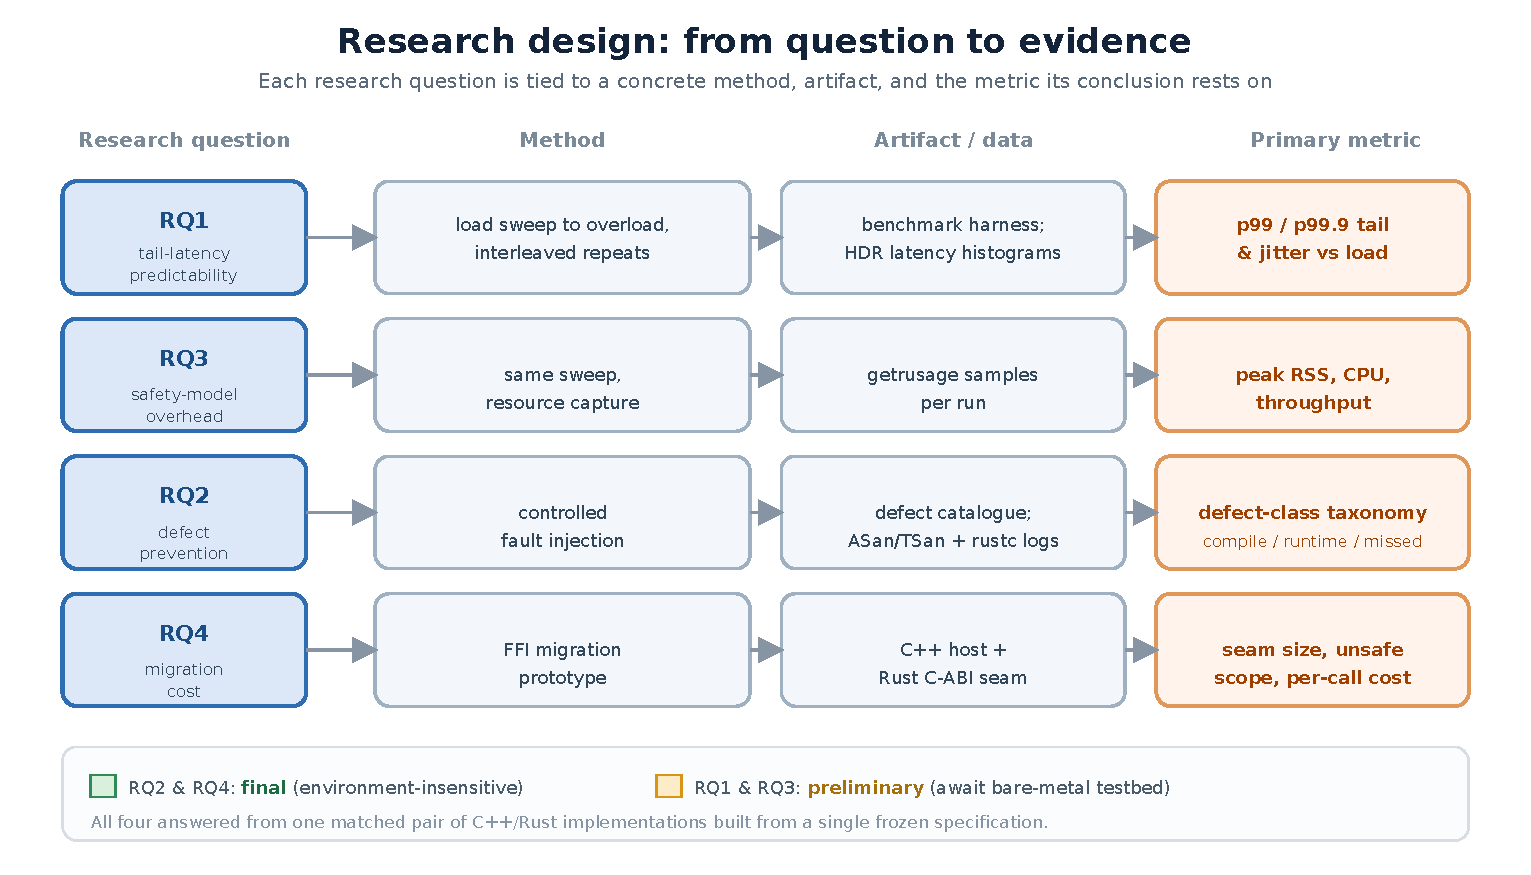
\includegraphics[width=\linewidth]{diagrams/pdf/10_rq_method_map.pdf}
\caption{The research design as a flow, showing for each research question the method, the
artifact and data it produces, and the primary metric its conclusion rests on. All four questions
are answered from one matched pair of C++/Rust implementations built from a single frozen
specification; RQ2 and RQ4 are environment-insensitive and reported as final, while RQ1 and RQ3
are preliminary until the bare-metal testbed campaign.\label{fig:rqmap}}
\end{figure}

\section{A constructive, comparative experiment}
The four research questions are causal and comparative: each asks how an outcome (tail
latency, prevented defects, resource use, or migration cost) depends on a single independent
variable, the implementation language. Answering such questions credibly requires that the
language be the \emph{only} systematic difference between the two objects under test. This
rules out the most common form of language comparison in the literature, in which two
independently written programs, or two unrelated projects, are measured and their differences
attributed to the language; such comparisons confound the language with the design, the
libraries, and the intent and skill of their authors. The thesis therefore adopts a
constructive (design-science) strategy: rather than locating two pre-existing systems, it
\emph{builds} the object of study as a matched pair of implementations derived from one frozen
specification, so that the comparison is between two encodings of the same design rather than
between two designs. The artifact, the specification, the two implementations, and the
benchmarking harness, is thus simultaneously the contribution of the thesis and the instrument
through which it is measured.

The experiment is empirical and quantitative where the questions admit numbers (RQ1, RQ3, and
the per-call cost of RQ4) and systematic-but-qualitative where they do not (the
kind-of-guarantee distinction in RQ2 and the API-design effort in RQ4). Evidence is
deliberately triangulated across three complementary methods rather than resting on a single
campaign, so that a weakness in any one method, for example the environment sensitivity of
tail-latency measurement, does not undermine the conclusions as a whole.

\section{Methods for the four research questions}
Table~\ref{tab:design} pairs each question with a method; this section states what each method
does and why it is appropriate.

\subsection{Performance measurement under a load sweep (RQ1, RQ3)}
RQ1 and RQ3 are answered by driving both implementations with one deterministic synthetic
workload across a sweep of offered load, from light load through saturation and into overload,
and recording latency and resource use at each level. Two design decisions make the
measurement sound. First, the load generator follows an \emph{open-loop} schedule with a fixed
intended send time per request, and latency is measured against that intended time rather than
against the moment the request is actually admitted; this is what corrects for coordinated
omission, the bias by which a naive closed-loop generator stalls together with the system and
silently fails to record the very requests that would have exposed the tail
(Chapter~\ref{chapter:background}). Second, the sweep is pushed past saturation deliberately:
the operationally decisive behaviour of a control plane is not its latency at nominal load but
the onset and shape of the overload cliff, and that is visible only once offered load exceeds
service capacity. Latency is captured in high-dynamic-range histograms configured identically
on both sides, and resource use (peak resident set size, CPU utilisation, throughput) is
sampled through the operating system, so that the same measurement apparatus is applied to both
languages.

\subsection{Controlled fault injection (RQ2)}
RQ2 asks which defect classes a language prevents, and it cannot be answered by measuring
defect-free code: the absence of a bug in a passing test says nothing about whether the
language would have caught it. The method is therefore adversarial, following the established
practice of software fault injection, in which representative faults are deliberately introduced
to assess how a system behaves in their presence~\cite{natella2016fault}. A catalogue of
representative C++ defects, drawn from the classes that afflict this subsystem
(Chapter~\ref{chapter:context}), is written \emph{deliberately}, each as a small self-contained
program flavoured with the domain (a stale pointer into the context map, a double release, a
mutation during iteration, an unsynchronised shared update). Each C++ defect is then built and
run under AddressSanitizer and ThreadSanitizer, recording which tool, if any, detects it and at
what stage; the analogous construct is written in safe Rust and compiled, recording the
compiler's outcome. Because the independent variable is again only the language while the
injected fault is held fixed, the difference in outcome, compile-time rejection, runtime
detection, or silent miss, is attributable to the language's guarantees rather than to the
specific bug. The result is a taxonomy rather than a performance number: the method establishes
the \emph{kind} of protection each language offers.

\begin{figure}
\centering
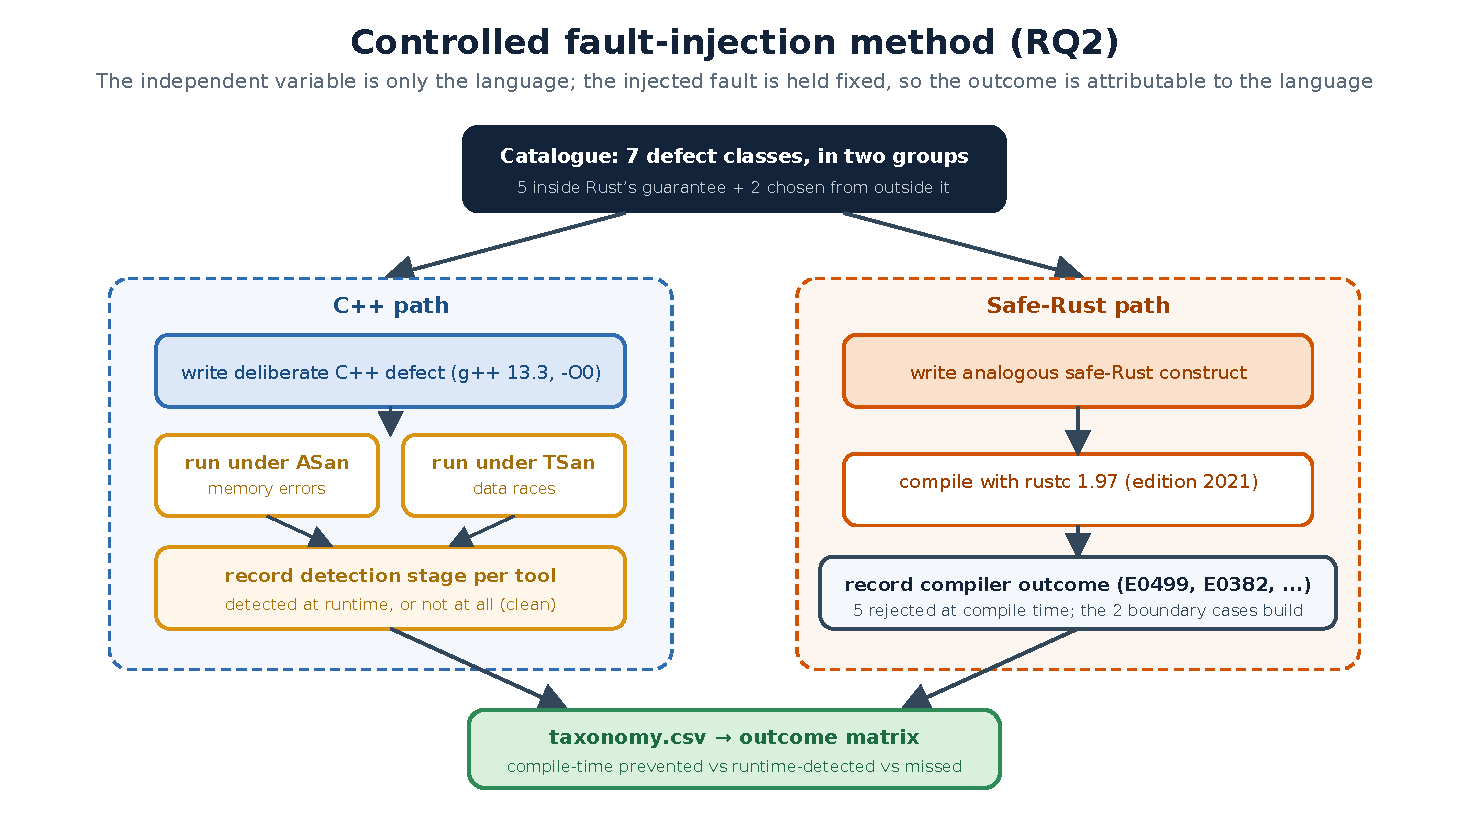
\includegraphics[width=\linewidth]{diagrams/pdf/14_fault_injection_method.pdf}
\caption{The controlled fault-injection method for RQ2. A fixed catalogue of representative
defect classes is confronted in two languages: each C++ defect is built and run under
AddressSanitizer and ThreadSanitizer to record the detection stage, while the analogous safe-Rust
construct is compiled to record the compiler's outcome. Because only the language varies while the
injected fault is held fixed, the difference in outcome is attributable to the language's
guarantees.\label{fig:faultmethod}}
\end{figure}

\subsection{Foreign-function-interface migration case study (RQ4)}
RQ4 concerns the practical cost of adopting Rust inside an existing C++ system, which is an
engineering question as much as a performance one. It is answered by constructing a working
prototype in the realistic direction of migration, an existing C++ host calling a Rust
component across a C application binary interface, and then measuring three quantities on it:
the \emph{size} of the interoperability seam (entry points, lines of code, dependencies), the
\emph{scope} of \texttt{unsafe} it forces (where the checked language is left, and whether the
safety-critical core is affected), and the \emph{per-call cost} of crossing the boundary
relative to the cost of the operation being invoked. The first two are structural and are read
off the code; the third is measured with the same histogram apparatus as the performance sweep.
This combination of a structural account and a quantitative cost measurement is what lets the
study separate the run-time cost of interoperability from its true cost, which lies in API
design and human learning.

\section{Fairness as a controlled-variable strategy}
Because every research question attributes a difference to the language, the validity of the
whole study depends on holding everything else equal, and fairness is treated as the study's
central experimental control rather than as an afterthought. It is enforced at several levels.
The \emph{specification} is frozen before any code is written and fixes the public API, the
state machine, the data structures and their algorithmic strategy, and the sharding and
concurrency model (Section~\ref{sec:fairness}). The \emph{run-time substrate} is equalised by
linking the same memory allocator on both sides and matching build-optimisation levels as
closely as the two toolchains allow. The \emph{workload} is produced by a driver that is
identical in structure across languages and, for a given seed and active-UE population, drives
both implementations through exactly the same sequence of operations, so that any latency
difference reflects how each language executes the same work rather than a difference in what
work is done. Where the two languages genuinely cannot express the same construct, the deviation
is not hidden but recorded in a forced-idiom log so it can be weighed explicitly in the
discussion. What remains uncontrolled, principally single-author skill asymmetry, is
acknowledged as a threat to validity (Chapter~\ref{chapter:discussion}) rather than claimed to
be eliminated.

\section{Statistical treatment of measurements}
Performance measurements are non-deterministic, so single-run numbers are avoided throughout.
Each configuration (language $\times$ allocator $\times$ load level) is measured over many
independent repeats, and the four variants are \emph{interleaved} within each repeat so that
slow drift, thermal effects, and background activity perturb them equally rather than biasing
one. Results are summarised by the median with a nonparametric bootstrap $95\%$ confidence
interval rather than by the mean with a standard deviation, because latency distributions are
heavy-tailed and skewed and a distribution-free interval on the median makes no normality
assumption. This follows established guidance on statistically rigorous performance evaluation,
which warns that reporting a single number invites conclusions that run-to-run variation does
not support~\cite{georges2007rigorous}. Tail percentiles (p99, p99.9, p99.99) are read from the
HDR histograms, whose logarithmic bucketing retains three significant figures of resolution
across the whole range so that high percentiles are not quantised away.

\section{Reproducibility and research artifacts}
The study is designed so that its results can be regenerated by a third party without access to
Nokia's proprietary code. The implementations are driven entirely by the public frozen
specification; the benchmarking harness, the fault catalogue and its runner, and the FFI
prototype are published together with the thesis; and every figure and table in the evaluation
is produced by a single script directly from the raw measurement logs, so that rerunning the
campaign on a different host regenerates the artifacts verbatim. The execution environment (CPU
model, kernel, compiler and toolchain versions, and the frequency and scheduling settings of
the testbed) is captured automatically alongside each result set, so that the conditions of a
measurement travel with its data. This separation of environment-sensitive results (the
performance sweep) from environment-insensitive ones (parity testing, fault injection, and the
FFI structure) is what lets the thesis label the former preliminary and the latter final
without ambiguity.

\section{Ethical and data-protection considerations}
The study processes no personal, subscriber, or operator-confidential data. All traffic is
synthetic and generated by the deterministic driver, the UE contexts contain only fabricated
identifiers and a fixed dummy security field, and the subsystem is modeled on, rather than
copied from, production code. There are therefore no privacy, consent, or data-retention
concerns, and the resulting artifacts can be released openly for reproduction.

\chapter{Problem Context: UE Context Management and Predictability\label{chapter:context}}

\section{The UE Context Management subsystem}
The subsystem under study is a UE Context Management service, modeled on a real Nokia
gNB-CU-CP service domain that owns the UE context lifecycle, RRC procedure
execution~\cite{3gpp38331}, and mobility/handover---the very functions the 3GPP architecture
assigns to the control-plane part of a disaggregated gNB, where the CU-CP hosts the RRC and the
control-plane part of PDCP and manages the UE context, delegating user-plane bearer handling to
the CU-UP over the E1 interface~\cite{3gpp38401,3gpp38300,3gpp38463}. It is a good representative
because it is core RAN L3 functionality,
performance- and latency-sensitive, inherently stateful and concurrent, and self-contained
enough to specify precisely and benchmark fairly. The modeled functionality includes UE
context creation and deletion, state transitions (e.g.\ idle to connected), signaling
message handling, and concurrent context lookup under load. Figure~\ref{fig:fsm} shows the
UE-context lifecycle state machine that both implementations encode identically; illegal
transitions (for example signaling an \texttt{Idle} context) return a typed error rather than
mutating state, and this state machine is exactly what the mixed workload of
Section~\ref{sec:workload} walks each UE through.

\begin{figure}
\centering
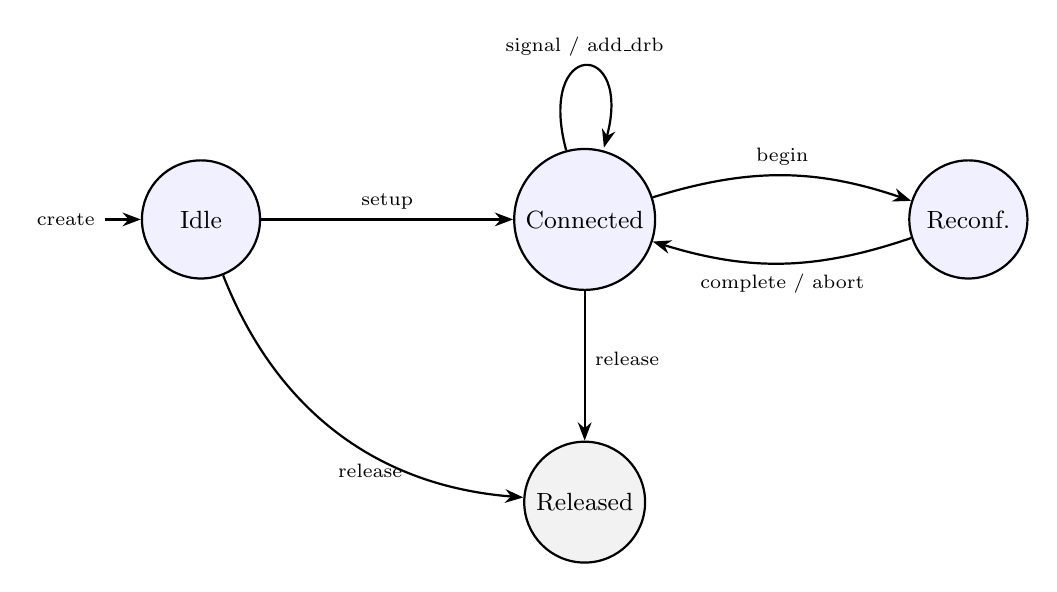
\begin{tikzpicture}[
    ->, >=Stealth, node distance=3.2cm, font=\small,
    every state/.style={draw, minimum size=1.5cm, fill=blue!6, thick},
    every edge/.style={draw, thick}
  ]
  \node[state, initial, initial text=\scriptsize create] (idle) {Idle};
  \node[state, right=of idle] (conn) {Connected};
  \node[state, right=of conn] (reconf) {Reconf.};
  \node[state, below=1.9cm of conn, fill=gray!10] (rel) {Released};

  \path (idle)  edge node[above,font=\scriptsize]{setup} (conn)
        (conn)  edge[bend left=18] node[above,font=\scriptsize]{begin} (reconf)
        (reconf) edge[bend left=18] node[below,font=\scriptsize]{complete / abort} (conn)
        (conn)  edge node[right,font=\scriptsize,pos=0.45]{release} (rel)
        (idle)  edge[bend right=32] node[below,font=\scriptsize,pos=0.6]{release} (rel);
  \path (conn) edge[loop above] node[font=\scriptsize]{signal / add\_drb} (conn);
\end{tikzpicture}
\caption{UE-context lifecycle state machine. \texttt{create} allocates a context in
\texttt{Idle}; \texttt{setup} connects it; \texttt{signal} and \texttt{add\_drb} are handled
in place while \texttt{Connected}; a reconfiguration/handover moves through
\texttt{Reconfiguring} and back on \texttt{complete} or \texttt{abort}; \texttt{release}
tears the context down. Operations invalid for the current state return an \texttt{OpError}
instead of changing state.\label{fig:fsm}}
\end{figure}

\paragraph{Representativeness and tractability.}
Two properties make UECM a good study object for a language comparison. It is
\emph{representative}: per-UE mutable state, a strict operation lifecycle, high inter-UE
concurrency, and the hard latency and reliability targets the 5G system places on control-plane
procedures~\cite{3gpp22261} are exactly the properties that make production
RAN control-plane code difficult, so conclusions about how a language handles them transfer to
the broader class of stateful, concurrent control-plane services. It is also \emph{tractable}:
the subsystem is small enough to specify precisely, implement faithfully in two languages, and
reason about in full, which is what makes a controlled, parity-tested comparison possible at
all. A larger or less well-bounded subsystem would improve external validity at the cost of the
internal validity on which a fair language comparison depends; UECM is chosen as the point that
keeps both within reach.

\paragraph{Operation set.}
The interface exercised by the study is deliberately small and lifecycle-oriented: create and
release a context; set up a connection (\texttt{Idle}$\rightarrow$\texttt{Connected}); handle an
in-session signaling message; add a data radio bearer; begin, complete, or abort a
reconfiguration/handover; and look up a context's state under concurrent load. Each operation is
total with respect to the state machine of Figure~\ref{fig:fsm}: an operation that is illegal in
the current state returns a typed error and leaves the context unchanged, rather than throwing
or corrupting state. This closed, well-typed operation set is what lets the same test vectors
and the same workload drive both implementations along identical paths
(Section~\ref{sec:parity}).

\section{Memory-safety and concurrency defect classes}
The defects that afflict C++ control-plane code of this kind fall into two families. The
\emph{memory-safety} family concerns the lifetime and bounds of objects: a \emph{use-after-free}
accesses storage that has already been released, a \emph{double-free} releases the same storage
twice, and a \emph{buffer overflow} reads or writes past the end of an allocation. The
\emph{concurrency} family concerns unsynchronised or ill-ordered access from multiple threads: a
\emph{data race} is a pair of unsynchronised accesses to the same location of which at least one
is a write, a \emph{deadlock} is a cyclic wait for locks, and \emph{iterator invalidation} is
the use of an iterator or reference into a container after a mutation has moved or freed the
underlying storage. What these share is that they are all \emph{silent} in C++: each is accepted
by the compiler and, on the paths ordinary tests happen to exercise, may appear to work,
surfacing only later as corruption, a crash, or an unpredictable latency spike---the same
memory-corruption classes that decades of security research have struggled to contain in C and
C++~\cite{szekeres2013sok}.

Each class has a natural incarnation in UE Context Management, which is why the subsystem is a
good vehicle for studying them:

\begin{itemize}
  \item \textbf{Use-after-free.} A signaling message holds a raw pointer or reference to a UE
        context that a concurrent \texttt{release} has already erased from the context map; the
        in-flight handler then dereferences freed storage.
  \item \textbf{Double-free.} A release path runs twice for the same UE, for example because a
        retransmitted release is not made idempotent, freeing the context's owned resources a
        second time.
  \item \textbf{Iterator invalidation.} Code iterates a context's data-radio-bearer list while
        adding or removing a bearer, so the iterator refers into storage the container has since
        reallocated.
  \item \textbf{Data race.} Two workers update the same context field, an activity counter or a
        state flag, without synchronisation, so the accesses race.
  \item \textbf{Unguarded shared mutation.} A context is shared by reference across threads and
        mutated without a lock or other discipline, a race whose root cause is the absence of any
        ownership rule for the shared state.
\end{itemize}

These five classes are exactly the catalogue injected in the fault-injection study of
Chapter~\ref{chapter:eval}: they both occur naturally in this subsystem and lie squarely within
the guarantees Rust claims to provide, which makes them the fairest test of whether that claim
holds. Deadlock and buffer overflow are described here for completeness but are not central to
the injected catalogue, the former because the shared-nothing design
(Chapter~\ref{chapter:design}) largely designs locks out of the hot path, and the latter because
neither implementation performs raw pointer arithmetic on the context store.

\begin{figure}
\centering
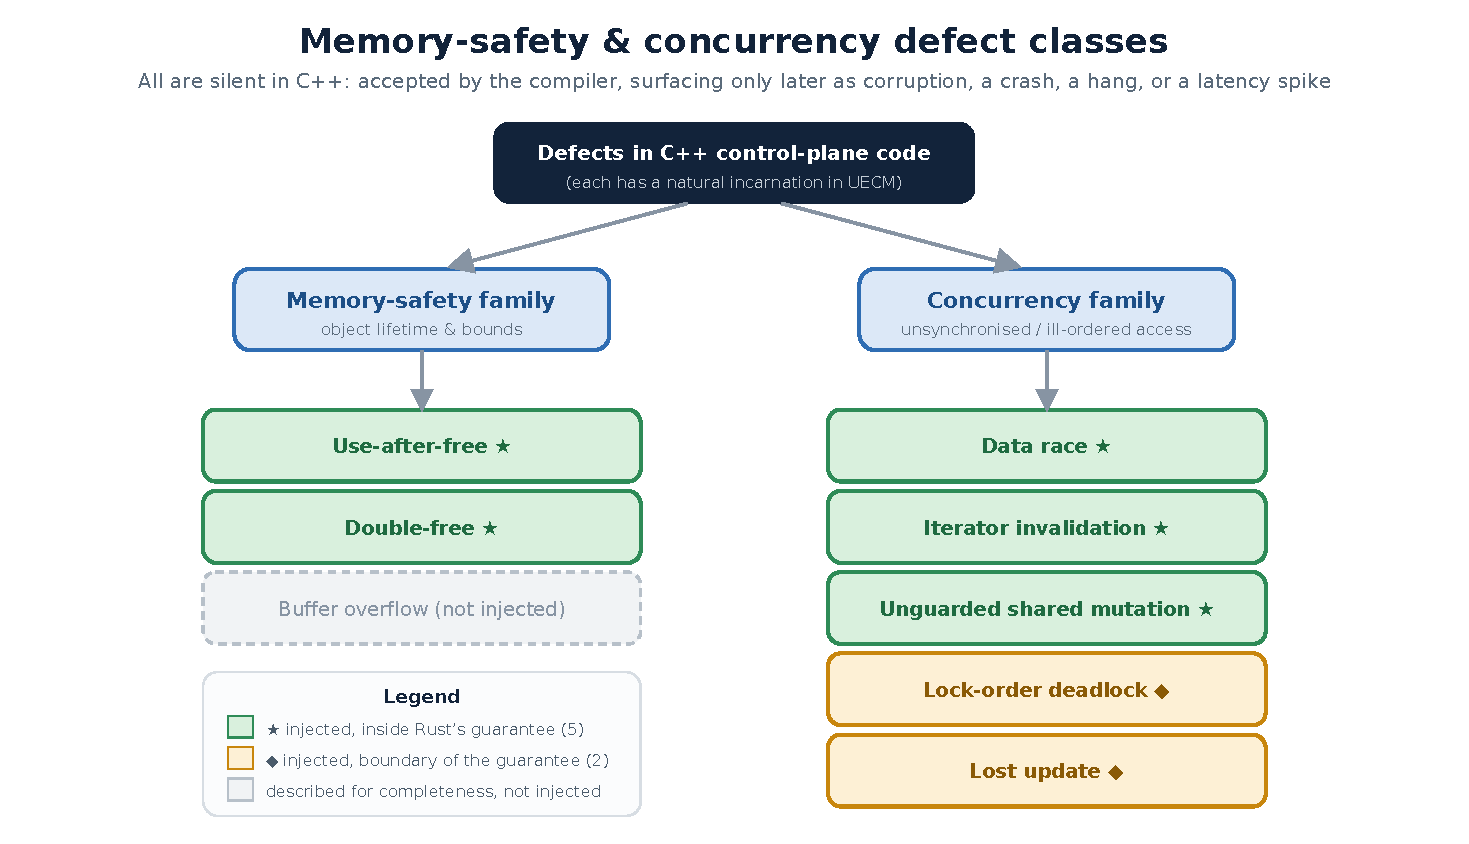
\includegraphics[width=0.92\linewidth]{diagrams/pdf/13_defect_families_tree.pdf}
\caption{The defect classes that afflict C++ control-plane code, split into a memory-safety
family (object lifetime and bounds) and a concurrency family (unsynchronised or ill-ordered
access). The five starred classes are the ones injected in the RQ2 fault-injection study; buffer
overflow and deadlock are described for completeness but are not central to the catalogue. All are
silent in C++, surfacing only later as corruption, a crash, or a latency spike.\label{fig:defectfamilies}}
\end{figure}

\section{Tail latency and predictability in RAN}
For deadline-driven RAN procedures, the meaningful performance question is how bad the slow
cases are, not how good the average is. This is the classic ``tail at scale'' problem: in a
system where a user-visible action fans out into many dependent operations, the slowest
component dominates the end-to-end experience, so the tail of the latency distribution, not
its mean, governs whether deadlines are met~\cite{dean2013tail}. The relevant time scale is
the microsecond: modern low-latency I/O and in-memory request handling operate in a regime
that existing systems, tuned for nanosecond and millisecond events, support
poorly~\cite{barroso2017microseconds}, which makes disciplined microsecond-level measurement
essential---the more so because much of the tail originates below the application, in hardware,
operating-system, and scheduling effects~\cite{li2014tales}. The study therefore characterises the full latency distribution, focusing on high
percentiles (p99, p99.9, p99.99), the maximum, and jitter, and on how these degrade as the
system approaches and exceeds saturation. Measuring these correctly requires care to avoid
coordinated-omission bias, which naive timing loops introduce when the system
stalls~\cite{tene_hdrhistogram}.

\paragraph{Deadlines, fan-out, and overload.}
Two features of the RAN setting turn tail latency from an academic nicety into the governing
metric. The first is \emph{fan-out}: a single user-visible action, a call setup or a handover,
decomposes into many dependent control-plane operations, and because the slowest of them gates
completion, a latency that is rare per operation becomes common per procedure~\cite{dean2013tail}.
The second is \emph{scale}: a busy site drives thousands of such procedures per second across
millions of connected devices, so a tail event that occurs once in a thousand operations is not
an edge case but a routine occurrence somewhere in the fleet at every instant. Compounding both
is queueing behaviour near capacity: as offered load approaches the service rate, queueing delay
grows super-linearly and the tail explodes, which is why a characterisation that stops at nominal
load misses the regime that actually decides service quality. This is the reasoning behind
sweeping the workload into overload and reporting the full latency distribution rather than the
mean (Chapter~\ref{chapter:eval}).

\begin{figure}
\centering
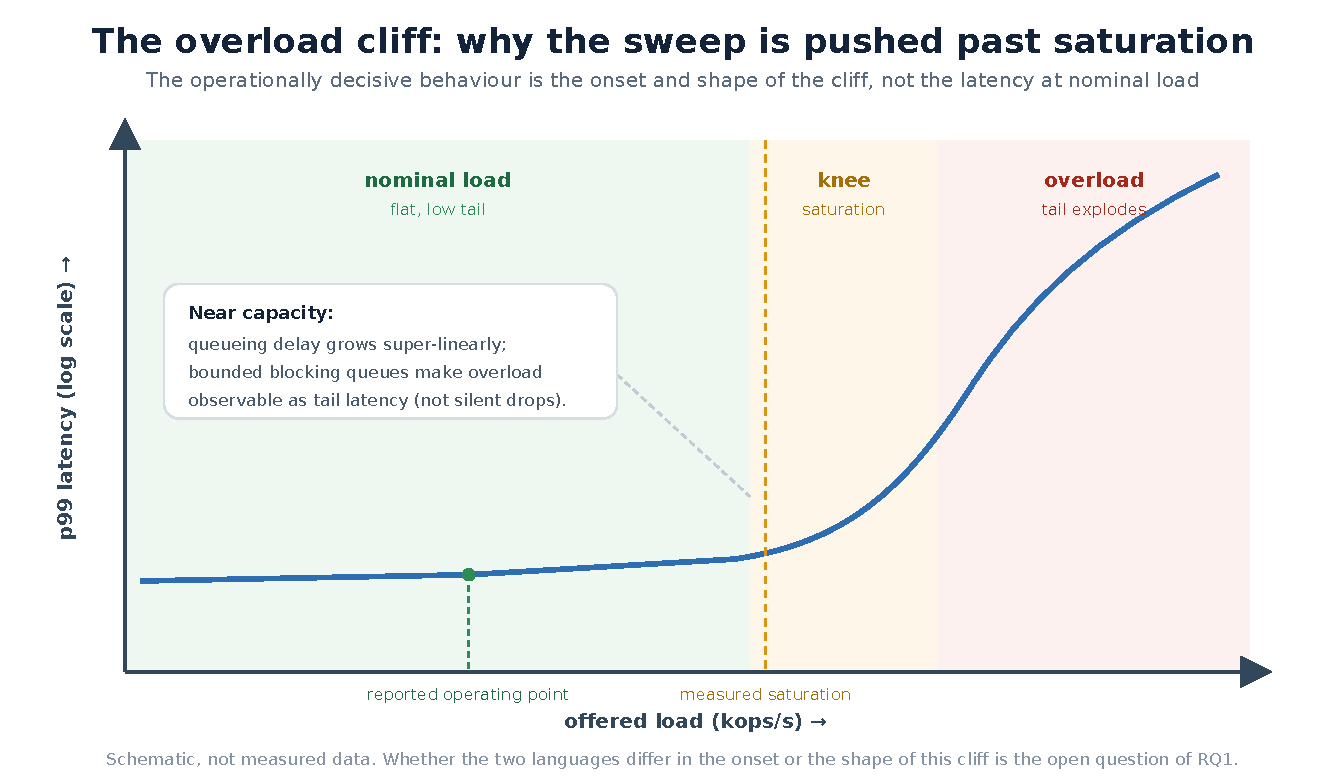
\includegraphics[width=0.9\linewidth]{diagrams/pdf/15_overload_cliff.pdf}
\caption{The overload cliff (schematic). Tail latency stays low and flat while offered load is
below service capacity, then climbs steeply once the system is driven past saturation and requests
queue behind the bounded, blocking queues. The operationally decisive behaviour is the onset and
shape of this cliff, which is why the load sweep is pushed beyond the saturation point rather than
stopping at nominal load.\label{fig:cliff}}
\end{figure}

\chapter{Objectives\label{chapter:objectives}}

\section{Deficiencies in existing comparisons}
Cross-language studies report that compiled systems languages such as C, C++, and Rust
achieve broadly similar time and energy efficiency, well ahead of managed and interpreted
languages~\cite{pereira2017energy}. The closest evidence in a networking context comes from
user-space packet processing: an idiomatic Rust 10~Gbit/s network driver executes many more
instructions per packet than its C reference yet runs only about $4\%$
slower~\cite{emmerich2019drivers}, suggesting Rust's safety checks are largely absorbed by
modern out-of-order CPUs. However, these comparisons are established mostly on general-purpose
or packet-forwarding benchmarks; they emphasise average performance or throughput, rarely
examine tail latency under overload for stateful concurrent control-plane workloads, do not
isolate the defect classes that a language prevents, and seldom quantify the cost of
incremental migration into an existing C++ codebase, a cost that qualitative adoption studies
report is dominated by the learning curve rather than by run-time
overhead~\cite{fulton2021adopting}. These are the gaps this thesis targets.

\section{Solution objectives}
The overarching objective is a fair, reproducible comparison of modern C++ and Rust for a RAN
control-plane subsystem, together with reusable artifacts and evidence-based guidance. It
decomposes into concrete objectives, each aligned with a research question so that progress is
traceable:

\begin{description}
  \item[O1 (predictability, RQ1)] Quantify and compare the latency distributions of the two
        implementations, focusing on the p99/p99.9 tail and jitter, across a load sweep that
        reaches overload, and identify where along that sweep, if anywhere, the languages
        diverge.
  \item[O2 (defect prevention, RQ2)] Determine, for a catalogue of defect classes
        representative of the subsystem, which are prevented at compile time in safe Rust and,
        for those that are not, at what stage and cost they are detected in C++.
  \item[O3 (overhead, RQ3)] Measure the resource cost, throughput, CPU utilisation, and memory
        behaviour, of each implementation under matched conditions, isolating any systematic
        penalty attributable to Rust's safety model.
  \item[O4 (migration, RQ4)] Build and measure a realistic incremental-adoption prototype,
        quantifying the size of the interoperability seam, the scope of \texttt{unsafe} it
        requires, and the per-call cost of crossing the language boundary.
  \item[O5 (artifacts and guidance)] Deliver a frozen specification, a parity-tested pair of
        implementations, a reproducible benchmarking framework, a defect-class taxonomy, and
        engineering guidelines that practitioners can reuse for language-selection decisions in
        cloud-native RAN evolution.
\end{description}

\section{Hypotheses}
The objectives are approached with three prior expectations, stated so that the evaluation can
confirm or refute them rather than merely describe results after the fact. \textbf{H1:} for
this workload the two languages are performance-equivalent in the operationally relevant region
below saturation, with any difference confined to the far tail. \textbf{H2:} safe Rust prevents
at compile time the memory-safety and concurrency defect classes that C++ leaves to
best-effort, after-the-fact detection. \textbf{H3:} the run-time cost of C++-to-Rust
interoperability is negligible relative to the cost of the operations invoked, so that the true
cost of incremental adoption is engineering effort rather than performance. These hypotheses are
revisited against the evidence in Chapter~\ref{chapter:discussion}.

\section{Success criteria}
The study is successful to the extent that it produces \emph{decision-grade} evidence, evidence
on which a practitioner could base a language choice, rather than merely a set of measurements.
Concretely this requires: that any performance comparison be reported with repeats and
confidence intervals so that a claimed difference is distinguishable from run-to-run noise; that
the defect-prevention result be demonstrated on concrete, compilable programs rather than argued
from language semantics alone; that the migration cost be read off a working prototype rather
than estimated; and that the whole be reproducible from published artifacts and a public
specification. Meeting these criteria is what distinguishes the contribution from the
general-purpose, average-case comparisons whose deficiencies motivate the work.

\section{Scope and boundaries}
The work focuses on a single representative subsystem studied under controlled, synthetic
conditions, and its boundaries are drawn deliberately to protect the internal validity of the
language comparison. In scope are the UE Context Management functionality of
Chapter~\ref{chapter:context}, the shared-nothing concurrency design, the load sweep to
overload, the fault-injection catalogue, and the FFI prototype. Explicitly out of scope are the
full gNB system and its remaining control-plane domains, PHY/L2 processing and the data-heavy
user plane, real captured traffic traces (as opposed to a spec-justified synthetic workload),
managed-language alternatives (excluded on the tail-latency grounds argued in
Chapter~\ref{chapter:background}), and production deployment and operational concerns such as
upgrade, observability, and multi-tenancy. These exclusions trade external validity for the
controlled conditions a fair language comparison needs, and each is revisited as a limitation in
Chapter~\ref{chapter:discussion}.

\chapter{Design and Implementation\label{chapter:design}}

\section{Shared specification: the fairness baseline}
\label{sec:fairness}
Before any code is written, a single language-agnostic specification is frozen: the public
API, the UE state machine, the data structures and their algorithmic strategy (e.g.\ a
sharded hash map keyed by UE identifier), the locking and sharding granularity, and the
concurrency model. Both implementations conform to this specification so that the comparison
measures language differences rather than design or skill asymmetry. The specification is
itself a deliverable and is the primary control against implementation bias.

\section{Conceptual model and concurrency design}
Two functionally equivalent implementations are developed against the shared specification:
a modern C++ version (C++23, STL, RAII, standard threading) and a Rust version (stable
toolchain, ownership-based memory model, safe concurrency). A single concurrency model is
used for both: a \emph{shared-nothing, thread-per-shard} model that mirrors how real RAN L3
partitions UE state, and mixing of async and thread-based models is intentionally avoided.

The UE-identifier space is partitioned into $N_{\text{shards}}$ shards (eight by default),
each owned by exactly one worker thread. Only that worker reads or mutates its shard's
contexts, so there is no shared mutable state between workers and no locks on context data.
Callers (load-generator threads) never touch context state directly; they submit request
messages to a shard's bounded multi-producer, single-consumer (MPSC) queue and wait on a
single-use completion handle to which the worker writes the result. The queue is
\emph{bounded and blocking}: when a shard's queue is full, submission blocks until space
frees up, which produces realistic queueing latency under overload and makes tail latency
the observable of the study (a non-blocking drop policy would hide overload). Requests to
the same shard are processed strictly first-in-first-out. This structure is what makes the
safe-concurrency comparison meaningful: the interesting machinery is the queue, the
completion handoff, and the ownership transfer of requests, rather than lock contention. The
only shared mutable state permitted is a single atomic counter used to stamp a per-context
activity sequence number, which is write-only bookkeeping that does not affect control flow.
Figure~\ref{fig:arch} shows this data flow.

\begin{figure}
\centering
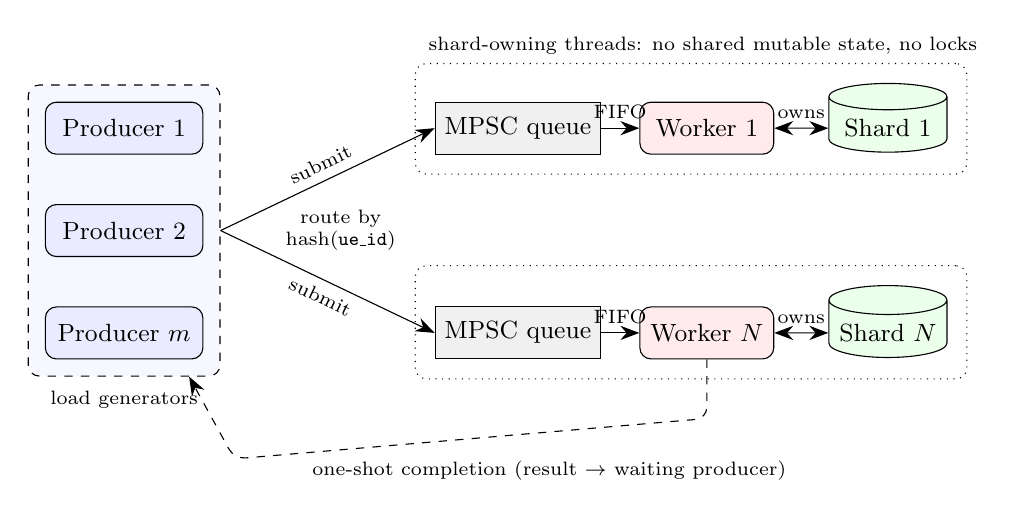
\begin{tikzpicture}[
    font=\small,
    prod/.style={draw, rounded corners, minimum width=2.0cm, minimum height=0.66cm, fill=blue!8},
    queue/.style={draw, minimum width=1.7cm, minimum height=0.66cm, fill=gray!12},
    worker/.style={draw, rounded corners, minimum width=1.7cm, minimum height=0.66cm, fill=red!8},
    store/.style={draw, cylinder, shape border rotate=90, aspect=0.25, minimum width=1.5cm, minimum height=0.85cm, fill=green!8},
    lane/.style={draw, dotted, rounded corners, inner sep=7pt},
    >={Stealth[length=2.4mm]}
  ]
  % producers, grouped in one box to avoid a tangle of crossing arrows
  \node[prod] (p1) at (0,1.3)  {Producer 1};
  \node[prod] (p2) at (0,0.0)  {Producer 2};
  \node[prod] (p3) at (0,-1.3) {Producer $m$};
  \begin{scope}[on background layer]
    \node[draw, dashed, rounded corners, fill=blue!3, fit=(p1)(p2)(p3), inner sep=6pt] (pg) {};
  \end{scope}
  \node[font=\scriptsize] at (0,-2.15) {load generators};

  % two representative shard lanes
  \node[queue] (q1) at (5.0,1.3)  {MPSC queue};
  \node[worker](w1) at (7.4,1.3)  {Worker 1};
  \node[store] (s1) at (9.7,1.3)  {Shard 1};
  \node[queue] (qn) at (5.0,-1.3) {MPSC queue};
  \node[worker](wn) at (7.4,-1.3) {Worker $N$};
  \node[store] (sn) at (9.7,-1.3) {Shard $N$};
  \begin{scope}[on background layer]
    \node[lane, fit=(q1)(s1)] (lane1) {};
    \node[lane, fit=(qn)(sn)] (lanen) {};
  \end{scope}
  \node[font=\scriptsize] at (7.35,2.35) {shard-owning threads: no shared mutable state, no locks};

  % submit: producer group -> each shard queue, routed by hash
  \node[font=\scriptsize, align=center] at (2.75,0) {route by\\ hash(\texttt{ue\_id})};
  \draw[->] (pg.east) -- (q1.west) node[midway, above, sloped, font=\scriptsize]{submit};
  \draw[->] (pg.east) -- (qn.west) node[midway, below, sloped, font=\scriptsize]{submit};

  % within-lane flow
  \draw[->]  (q1) -- node[above, font=\scriptsize]{FIFO} (w1);
  \draw[->]  (qn) -- node[above, font=\scriptsize]{FIFO} (wn);
  \draw[<->] (w1) -- node[above, font=\scriptsize]{owns} (s1);
  \draw[<->] (wn) -- node[above, font=\scriptsize]{owns} (sn);

  % one-shot completion: clean orthogonal return path below everything
  \draw[->, dashed, rounded corners=4pt]
      (wn.south) -- ++(0,-0.75) -- (1.4,-2.9) -- ($(pg.south east)+(-0.4,0)$);
  \node[font=\scriptsize] at (5.4,-3.05) {one-shot completion (result $\rightarrow$ waiting producer)};
\end{tikzpicture}
\caption{Shared-nothing, thread-per-shard architecture. Producers submit request messages to a
shard's bounded, blocking MPSC queue (selected by a pinned hash of the \texttt{ue\_id}) and wait
on a single-use completion handle; each shard is read and written by exactly one worker thread,
so there are no locks on context state. Blocking on a full queue is what makes overload
observable as tail latency.\label{fig:arch}}
\end{figure}

\section{Architectural choices and technology stack}
The C++ side uses CMake with Ninja, the standard library, and \texttt{std::thread}; the Rust
side uses Cargo and the stable toolchain. To keep the comparison a language comparison
rather than an allocator comparison, both link the same memory allocator: C++ links the
system \texttt{jemalloc} and Rust installs a \texttt{jemalloc} global allocator (from
\texttt{tikv-jemallocator}), with a system-allocator build retained on each side as a
control. Both record latency through the same high-dynamic-range (HDR) histogram
algorithm~\cite{tene_hdrhistogram}, configured identically (range $[1\,\text{ns},
3.6\,\text{s}]$, three significant figures); Rust uses the canonical \texttt{hdrhistogram}
crate and C++ uses a header-only port of the same bucketing algorithm, validated against a
known distribution. Build optimisation is matched as closely as the two toolchains allow:
the Rust release profile is pinned to \texttt{opt-level~=~2} to match the C++ \texttt{-O2}
build.

\section{Implementation details}
Both implementations follow the frozen specification field-for-field. Each UE context stores
its identifier, lifecycle state (a four-value enumeration \texttt{Idle}, \texttt{Connected},
\texttt{Reconfiguring}, \texttt{Released}), serving cell, RRC transaction id, a fixed 32-byte
dummy security context, a dynamic list of up to eight data radio bearers, and two counters.
The data radio bearer list is deliberately a growable container (\texttt{std::vector} /
\texttt{Vec}) rather than a fixed array, so that the allocator study (RQ3) observes realistic
per-context allocation. Reads return an immutable snapshot (a \texttt{UeContextView}) copied
out of the worker rather than a reference into live shard state, which preserves the
shared-nothing guarantee and keeps the two implementations semantically identical.

\begin{figure}
\centering
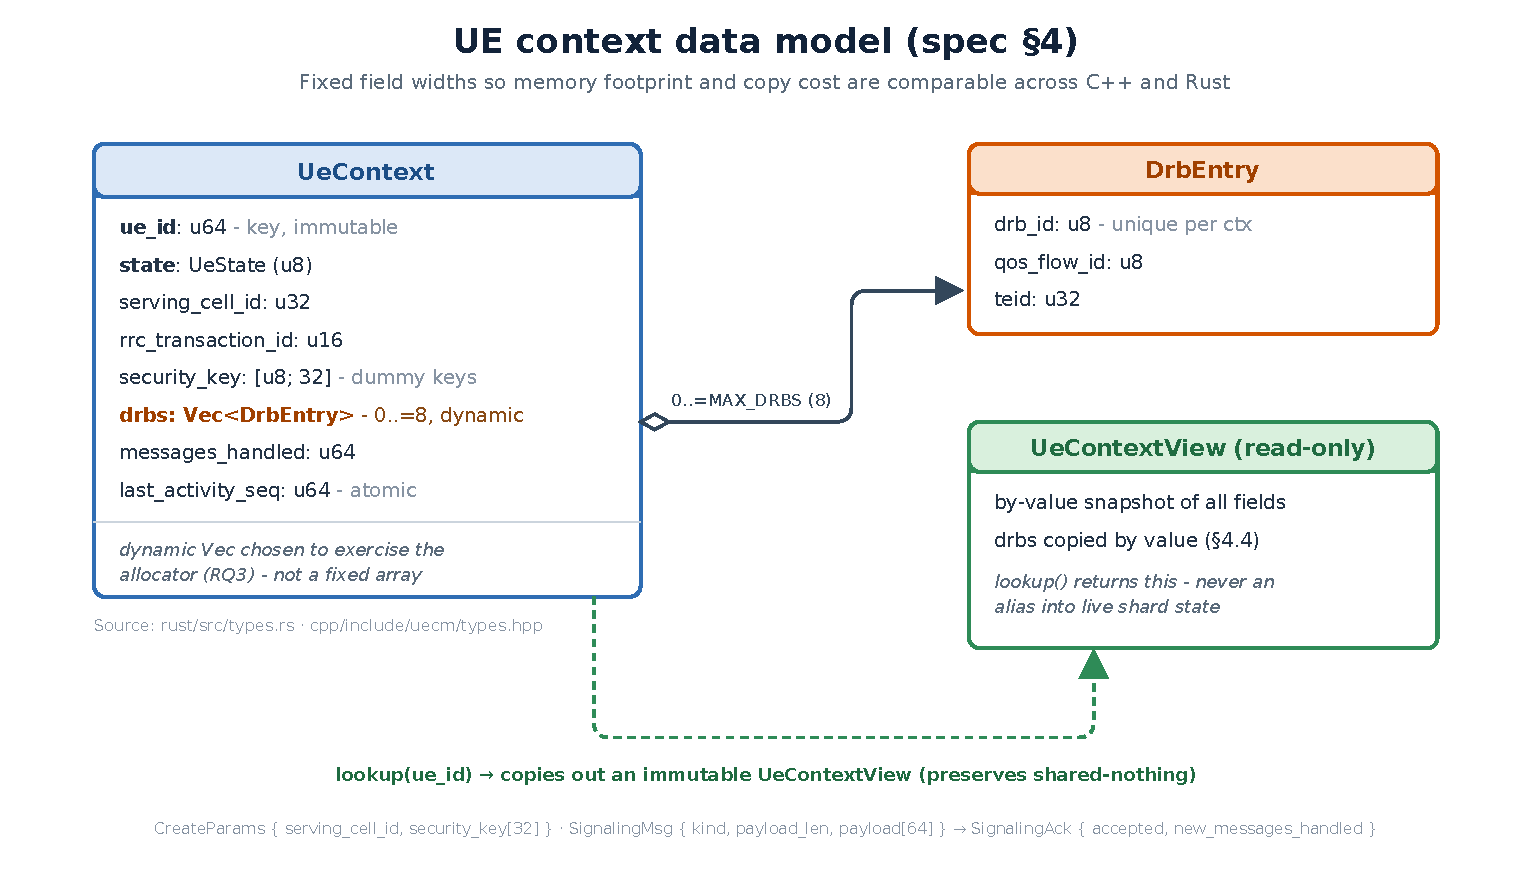
\includegraphics[width=0.92\linewidth]{diagrams/pdf/05_data_model.pdf}
\caption{The UE-context data model shared by both implementations. Field widths are fixed so that
memory footprint and copy cost are comparable across languages; the data-radio-bearer list is a
dynamic \texttt{Vec}/\texttt{std::vector} on purpose, to exercise the allocator for RQ3.
\texttt{lookup} returns an immutable \texttt{UeContextView} copied out by value rather than an
alias into live shard state, preserving the shared-nothing guarantee.\label{fig:datamodel}}
\end{figure}

\paragraph{Shard selection and the intra-shard store.}
To prevent the standard library hashers from becoming an accidental language advantage, both
sides pin their hashing. Shard assignment applies the SplitMix64 finalizer to the
\texttt{ue\_id} before reducing modulo the shard count, avoiding skew for sequential
identifiers. The per-shard container is each language's standard hash map
(\texttt{std::unordered\_map} / \texttt{std::collections::HashMap}) but keyed through a
pinned FNV-1a 64-bit hash over the eight little-endian bytes of the identifier; a test checks
that the Rust \texttt{BuildHasher} produces a digest bit-identical to the reference
\texttt{fnv1a\_64}. Both maps reserve an initial capacity at start-up so that steady-state
measurements are not perturbed by rehashing.

\paragraph{Language-forced idioms.}
Where the two languages must diverge to satisfy the same requirement, the deviation is
recorded in the specification's forced-idiom log so it can be weighed in the discussion. The
result type is \texttt{std::expected<T, OpError>} in C++23 and the idiomatic
\texttt{Result<T, OpError>} in Rust. A request is a move-only tagged struct carrying a
\texttt{std::promise} completion in C++, and an \texttt{enum} whose variants each carry a
typed one-shot sender in Rust, so the Rust caller needs no runtime variant dispatch on the
response. The bounded blocking queue is a hand-written \texttt{mutex}-plus-condition-variable
structure in C++ and a \texttt{sync\_channel} in Rust; the one-shot completion is
\texttt{std::promise}/\texttt{std::future} in C++ and a per-request channel in Rust.

\paragraph{Safety story.}
The Rust library contains \emph{no} \texttt{unsafe} code: safe Rust guarantees data-race
freedom at compile time through the \texttt{Send}/\texttt{Sync} traits, so no runtime
sanitizer is needed to establish it. The C++ implementation performs no manual memory
management beyond STL containers and was verified data-race free under ThreadSanitizer. This
asymmetry, a compile-time guarantee on one side versus an instrumented test on the other, is
exactly what the fault-injection study of Chapter~\ref{chapter:eval} quantifies.

\section{Public API and operation semantics}
Both implementations expose the same small, lifecycle-oriented API against the shared
specification, so that the surface a caller sees is identical up to each language's naming
conventions. A service is created with a fixed shard count and a per-shard queue bound;
thereafter callers invoke context operations, create, setup, handle-signaling, add-bearer,
reconfigure begin/complete/abort, release, and state lookup, each identified by the target
\texttt{ue\_id}. Every operation is \emph{total} and \emph{typed}: it returns a success value or
a typed \texttt{OpError} drawn from a closed enumeration (for example \texttt{NotFound},
\texttt{InvalidState}, \texttt{BearerLimit}), and an operation that is illegal for the context's
current state (Figure~\ref{fig:fsm}) returns the corresponding error and leaves the context
unchanged rather than mutating it or signaling failure out of band. This choice matters for
fairness as much as for correctness: because neither implementation uses exceptions or error
codes as a hidden control-flow channel, the cost and the control flow of the failure path are
visible and identical on both sides, and the same conformance vectors (Section~\ref{sec:parity})
can assert op-for-op agreement on both the returned value and the resulting state.

\section{Request lifecycle and the completion handoff}
The end-to-end path of a single operation is the machinery the study actually measures, so it is
worth stating precisely. A caller constructs a request carrying the operation, its arguments, and
a single-use completion handle, and computes the target shard from a pinned hash of the
\texttt{ue\_id}. It submits the request to that shard's bounded MPSC queue: if the queue has
space the request is enqueued and the caller blocks on the completion handle; if the queue is
full the \emph{submission} blocks until space frees, which is the point at which offered overload
becomes observable as queueing latency rather than being silently dropped. The shard's single
worker dequeues requests in strict FIFO order, executes the operation against its exclusively
owned store, writes the result (a success value or an \texttt{OpError}, and for reads an
immutable \texttt{UeContextView} copied out of live state) into the completion handle, and moves
on to the next request. Ownership of the request, and of any heap data it carries, is
transferred to the worker on submit and is never shared, which is what upholds the
shared-nothing invariant end to end. Latency is measured across this entire path, from intended
send time to completion, so that it includes queueing delay under load and reflects the same
cross-thread round-trip on both sides.

\begin{figure}
\centering
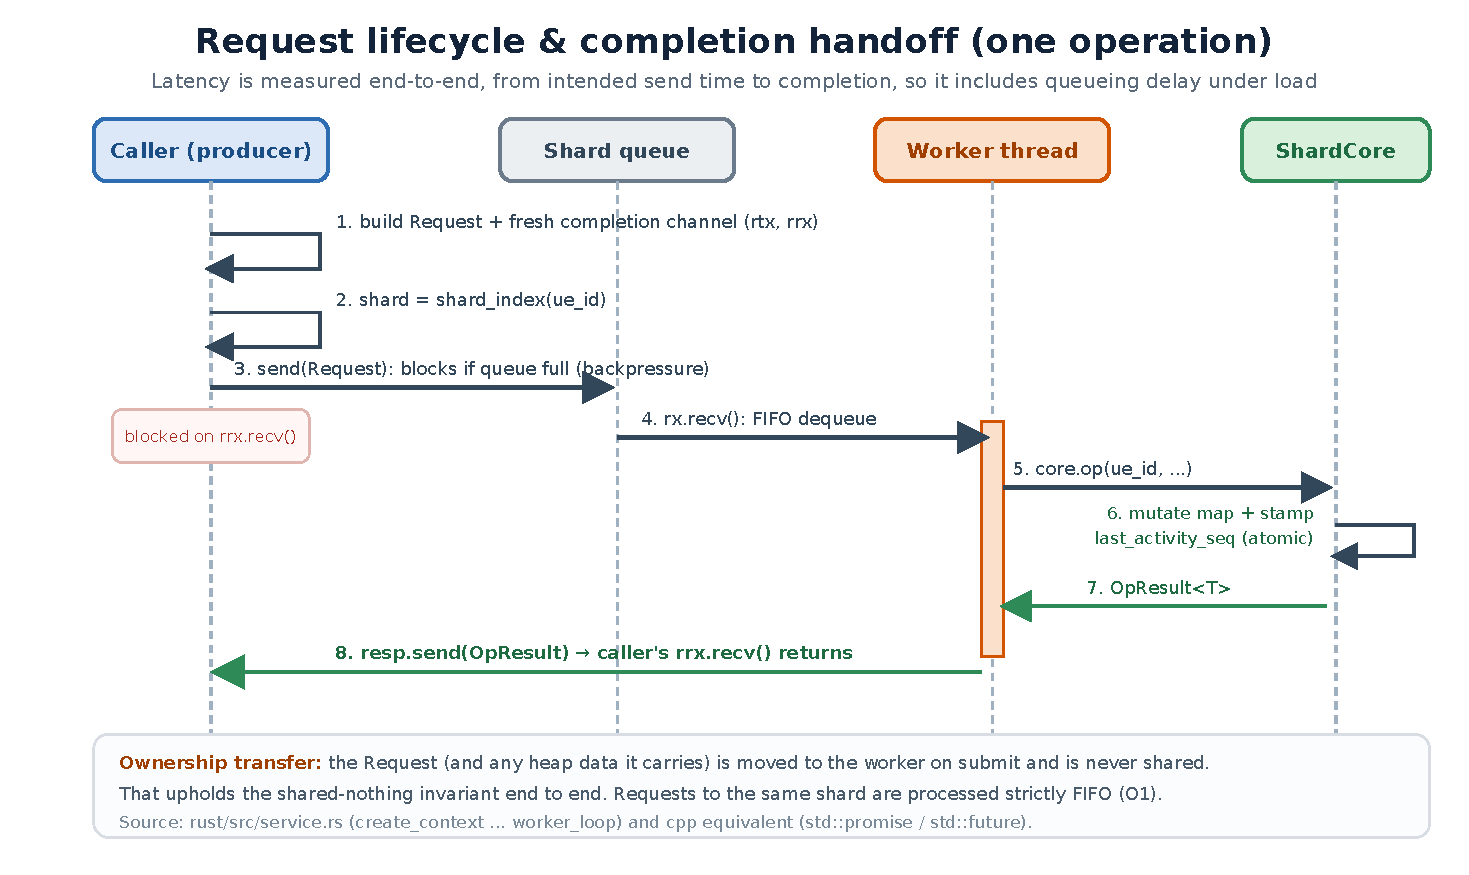
\includegraphics[width=\linewidth]{diagrams/pdf/04_request_lifecycle_sequence.pdf}
\caption{The end-to-end path of a single operation and the completion handoff. The caller builds
a request with a single-use completion handle, routes it by \texttt{shard\_index(ue\_id)} to the
owning shard's bounded queue (blocking if it is full), and waits; the shard's single worker
dequeues in FIFO order, executes the operation against its exclusively owned store, and writes the
result back to the completion handle. Ownership of the request is transferred to the worker on
submit and never shared. Latency is measured across the whole path.\label{fig:reqlifecycle}}
\end{figure}

\section{Parity verification}
\label{sec:parity}
Because the whole comparison rests on the two versions being functionally identical, parity
is tested rather than assumed. A language-neutral conformance suite expresses test vectors as
sequences of operations with their expected results and an expected post-state summary; a
runner in each language executes the vectors and emits a canonical transcript, and the two
transcripts are diffed for op-for-op agreement. The seeded suite covers the full error model,
the reconfiguration begin/complete/abort paths, data-radio-bearer fill and overflow, and
shard-assignment determinism; both implementations currently pass and agree. The benchmark
workloads add a second, independent parity signal: the mixed workload's per-operation-kind
counts are verified to be identical across languages for a given seed and active-UE
population, confirming that both implementations are driven along exactly the same code paths.

\chapter{Experimental Setup and Evaluation\label{chapter:eval}}

\section{Testbed configuration\label{sec:testbed}}
Performance experiments run on a dedicated bare-metal Linux host with identical hardware for
both implementations, following a documented protocol that removes avoidable sources of
tail-latency noise. The benchmark process is pinned to isolated physical cores with
\texttt{taskset}; the frequency governor is set to \texttt{performance}; turbo/boost and,
where per-core behaviour is measured, simultaneous multithreading are disabled; and an
initial warm-up fraction of each run is discarded so that cache- and allocator-cold effects
do not pollute steady state. Each sweep point is repeated many times and reported as a median
with a dispersion measure rather than as a single run, and the four language$\times$allocator
variants are interleaved within each repeat so that thermal or background drift affects them
equally. The environment (CPU model, kernel, compiler versions, governor and turbo state) is
captured automatically alongside the results, and the full configuration and scripts are
published for reproducibility. Functional work (parity testing, fault injection, and the FFI
prototype) is environment-insensitive and was carried out on a WSL2 development machine, but
the headline latency and resource figures are produced only on the bare-metal testbed, since
WSL2 does not expose the frequency and scheduling controls the protocol requires.

\section{Workload and evaluation measurements\label{sec:workload}}
A synthetic but spec-justified telecom workload is generated by a deterministic driver shared
in structure by both implementations, so that the two versions are exercised along identical
code paths. Two workloads are provided. The \emph{signal} workload preloads a population of
connected UEs and then hammers the \texttt{handle\_signaling} hot path, isolating steady-state
per-message latency. The \emph{mixed} workload is a pinned RAN lifecycle generator that walks
each UE through a realistic procedure sequence, context creation, connection setup, signaling,
bearer setup, reconfiguration/handover (begin/complete/abort), and release, using a fixed
SplitMix64 draw order and a per-slot expected-state model so that every emitted operation is
valid. Because the draw order is fixed, the per-operation-kind counts are identical in C++ and
Rust for a given active-UE population and seed, which doubles as the parity signal described in
Section~\ref{sec:parity}. The control parameters are the target event rate and the number of
active UEs, swept from nominal load through saturation and overload; a fixed send schedule with
histogram correction is used so that coordinated-omission bias is avoided when the system
stalls~\cite{tene_hdrhistogram}. Three measurement campaigns are run: a load sweep for
performance, the fault-injection study, and an FFI migration prototype.

\section{Data collection and metrics}
The study records latency predictability (per-event mean, median, p99/p99.9/p99.99, and
maximum latency, plus jitter), throughput (sustained events/sec and throughput at a fixed
latency service-level objective (SLO)), resource use (CPU utilisation, memory over time, allocation patterns),
concurrency robustness, safety (defect classes prevented at compile time vs runtime), and
software-quality proxies (lines of code, cyclomatic complexity, and the count and scope of
Rust \texttt{unsafe} blocks). Following established guidance on statistically rigorous
performance evaluation, each configuration is measured over many independent, interleaved
repeats and reported as a median with a bootstrap $95\%$ confidence interval rather than as a
single number, so that run-to-run non-determinism does not lead to unsupported
conclusions~\cite{georges2007rigorous}. Only synthetic data is used, so no personal,
subscriber, or confidential data is processed.

\section{Evaluation data}
The collected dataset consists of per-event latency histograms, throughput and resource-use
time series for each load level and language, the per-defect outcomes of the fault-injection
runs, and the interop measurements of the FFI prototype. A full preliminary campaign
(two languages $\times$ two allocators $\times$ eight load levels $\times$ four repeats) has
been captured on the development environment and is used below to exercise the analysis
pipeline; the performance figures will be refreshed with testbed-grade numbers by rerunning
the same scripts on the host of Section~\ref{sec:testbed}.

\section{Evaluation results}
The performance and resource results below are preliminary (development-environment)
measurements; the safety and migration results do not depend on testbed hygiene and are final.

\subsection{Performance (RQ1, RQ3)}
The hypothesis is that Rust and C++ achieve similar mean throughput but may differ
measurably in tail latency and jitter under overload, and that any safety-model overhead in
Rust is small in realistic workloads. The evaluation reports where, if anywhere, each
language wins and by how much, across the load sweep up to and beyond saturation.

The figures and tables in this section are generated by a single reproducible script
(\texttt{bench/plot\_figures.py}) directly from the raw measurement logs, so they can be
regenerated verbatim once the campaign is rerun on the bare-metal testbed of
Section~\ref{sec:testbed}. The numbers reported here are \emph{preliminary}, collected on the
development environment (WSL2), which is explicitly not testbed-grade for tail-latency claims;
they are included to exercise the full measurement-and-analysis pipeline and to illustrate the
kind of evidence each research question will rest on. Each point aggregates four interleaved
repeats, and shaded bands are nonparametric bootstrap $95\%$ confidence intervals on the
median.

Table~\ref{tab:latency} summarises the per-operation latency distribution at a sustained load
of $16$~kops/s, a representative operating point comfortably below the onset of overload on
this machine. Across
the four build variants the medians (p50) agree to within a few microseconds and the p99
values lie within roughly $20\%$ of one another; the languages diverge only in the far tail
(p99.9 and max), where allocator choice matters as much as language.

\begin{table}
\centering
\caption{Per-operation latency at a sustained load of $16$~kops/s (mixed RAN-lifecycle
workload, $8$ shards). Values in microseconds, medians over four repeats. Preliminary,
development-environment (WSL2) measurements.\label{tab:latency}}
\begin{tabular}{l r r r r r r}
\hline\hline
Variant & mean & p50 & p90 & p99 & p99.9 & max \\
\hline
C++ (system alloc) & \mci{217.2}{163.8}{237.2} & \mci{355.1}{289.3}{389.4} & \mci{674.3}{395.3}{1538.0} & \mci{2170}{910}{5594} \\
C++ (jemalloc) & \mci{225.8}{181.1}{261.2} & \mci{410.1}{305.7}{11280.4} & \mci{1188}{544}{14213} & \mci{3590}{1472}{16291} \\
Rust (system alloc) & \mci{214.3}{191.6}{238.8} & \mci{376.3}{330.2}{3629.1} & \mci{1068}{504}{6955} & \mci{2404}{1129}{9667} \\
Rust (jemalloc) & \mci{208.4}{193.7}{223.1} & \mci{388.9}{342.3}{478.0} & \mci{763.4}{479.5}{4272.1} & \mci{2804}{1114}{7606}
\\
\hline
\end{tabular}
\end{table}

Figure~\ref{fig:latency-load} plots p99 latency against offered load. All variants track a
low, flat tail (a few hundred microseconds) up to roughly $50$~kops/s, beyond which the
blocking-backpressure design pushes the system into overload and end-to-end latency, which
includes time spent waiting in the bounded queues, climbs steeply. The onset and shape of this
overload cliff, rather than the behaviour deep in saturation (which is dominated by the WSL2
scheduler here), is the quantity of interest, and is exactly what the bare-metal campaign will
pin down.

\begin{figure}
\centering
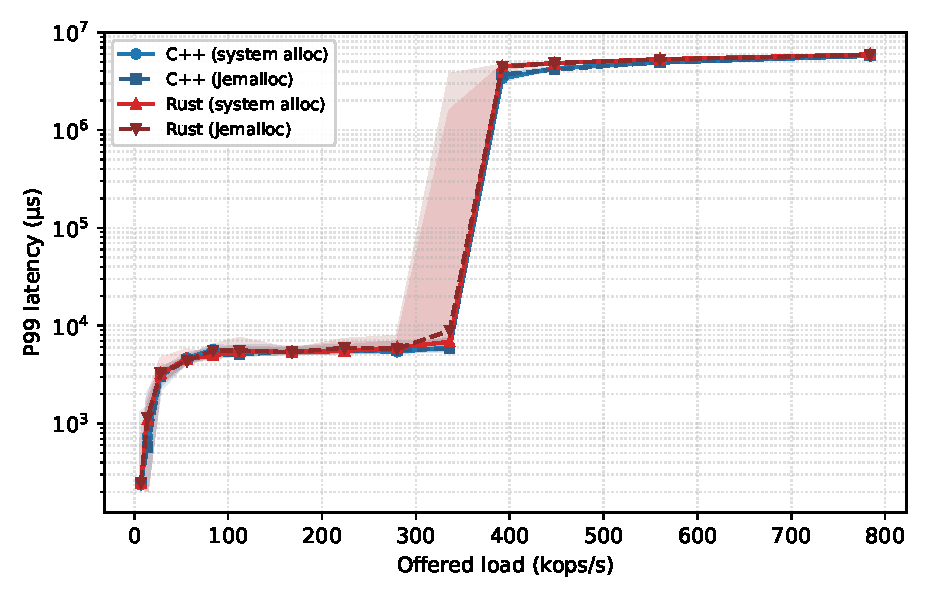
\includegraphics[width=0.82\linewidth]{figures/fig_latency_vs_load.pdf}
\caption{Tail latency (p99) versus offered load for the four build variants. Lines are medians
over four repeats; shaded bands are bootstrap $95\%$ CIs. Log-scaled $y$-axis. Preliminary
(WSL2) data.\label{fig:latency-load}}
\end{figure}

Figure~\ref{fig:throughput-load} shows achieved throughput against offered load. Every variant
follows the ideal line until it saturates near $40$--$45$~kops/s and then falls back as
producers block on full queues, confirming that the divergence in Figure~\ref{fig:latency-load}
coincides with the throughput knee rather than with any language-specific effect at low load.

\begin{figure}
\centering
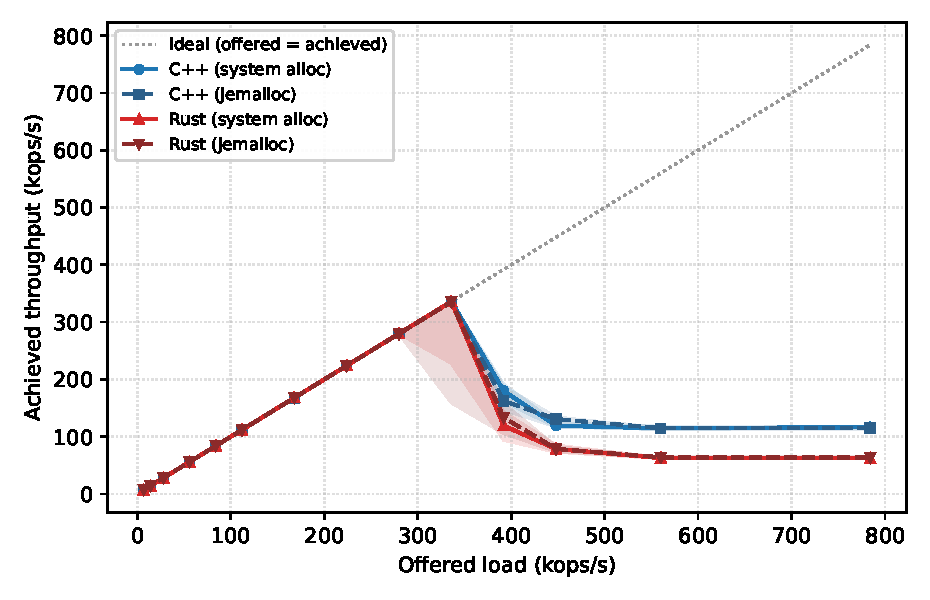
\includegraphics[width=0.82\linewidth]{figures/fig_throughput_vs_load.pdf}
\caption{Achieved throughput versus offered load. The dotted line marks the ideal
offered-equals-achieved regime. Preliminary (WSL2) data.\label{fig:throughput-load}}
\end{figure}

Figure~\ref{fig:tail} isolates the shape of the distribution at the $16$~kops/s sustained
load by plotting latency against percentile. The curves are almost indistinguishable through
p99 and separate only at p99.9, illustrating that the interesting differences between the two
languages live entirely in the tail, which is precisely why a percentile-aware methodology
(HDR histograms with coordinated-omission correction) is used throughout.

\begin{figure}
\centering
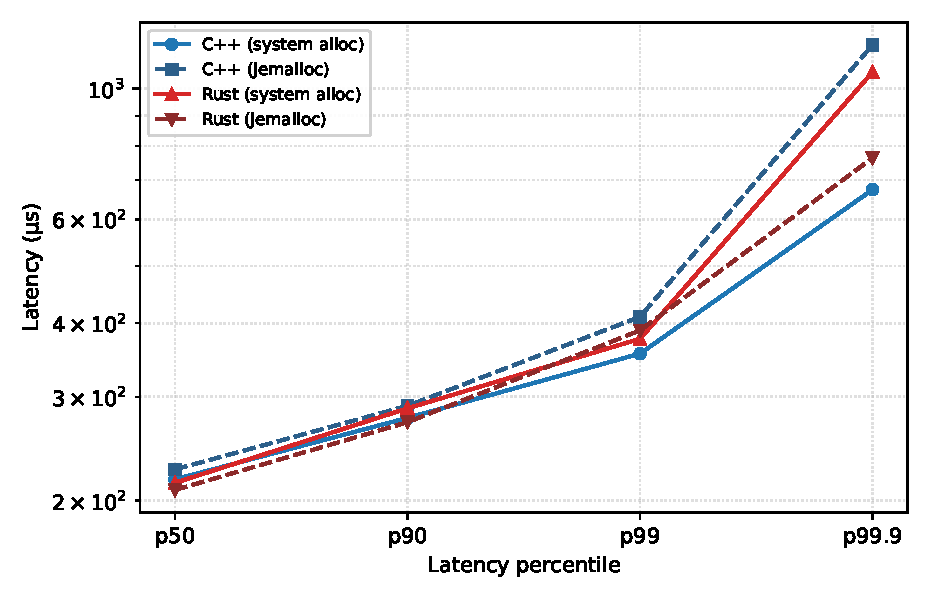
\includegraphics[width=0.82\linewidth]{figures/fig_tail_percentiles.pdf}
\caption{Latency by percentile at $16$~kops/s sustained load; log-scaled $y$-axis. The four
variants coincide through p99 and diverge only in the far tail. Preliminary (WSL2)
data.\label{fig:tail}}
\end{figure}

For RQ3, Table~\ref{tab:resource} and Figure~\ref{fig:resources} report resource use at the
same sustained load. Peak resident set size is modest and similar across variants (single-digit
to low-double-digit MiB); the system-allocator C++ build is the leanest, and jemalloc trades a
few extra megabytes of RSS for its tail-latency benefits. CPU utilisation is comparable across
all four, consistent with the shared thread-per-shard design doing the same work in each
language.

\begin{table}
\centering
\caption{Resource use at a sustained load of $16$~kops/s: achieved throughput, peak RSS, and
total CPU utilisation. Medians over four repeats. Preliminary, development-environment (WSL2)
measurements.\label{tab:resource}}
\begin{tabular}{l r r r}
\hline\hline
Variant & throughput (kops/s) & peak RSS (MiB) & CPU (\%) \\
\hline
C++ (system alloc) & \mci{27.99}{27.99}{27.99} & \mci{9.4}{9.4}{9.5} & \mci{66.8}{65.8}{68.2} \\
C++ (jemalloc) & \mci{27.95}{27.95}{27.96} & \mci{65.9}{65.9}{65.9} & \mci{64.6}{63.4}{66.1} \\
Rust (system alloc) & \mci{27.99}{27.99}{27.99} & \mci{11.2}{11.1}{11.3} & \mci{63.3}{62.2}{66.0} \\
Rust (jemalloc) & \mci{27.95}{27.92}{27.96} & \mci{67.2}{65.4}{67.3} & \mci{63.0}{62.4}{64.5}
\\
\hline
\end{tabular}
\end{table}

\begin{figure}
\centering
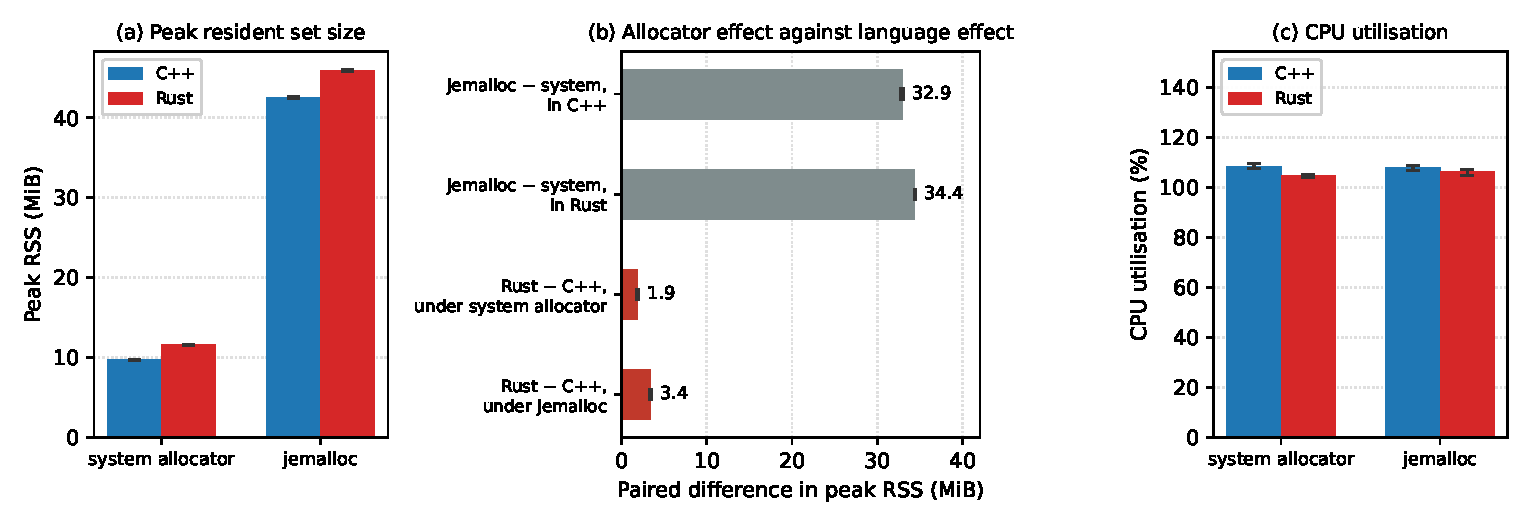
\includegraphics[width=\linewidth]{figures/fig_resources.pdf}
\caption{Peak resident set size (left) and CPU utilisation (right) per build variant at
$16$~kops/s. Preliminary (WSL2) data.\label{fig:resources}}
\end{figure}

\subsection{Safety via fault injection (RQ2)}
Instead of claiming that Rust has no bugs, a catalogue of five classic C++ defects is
deliberately injected: use-after-free, double-free, iterator invalidation, data race, and
unguarded shared mutation. Each defect is a small, self-contained program flavoured with the
subsystem's domain (a stale pointer into the context map, releasing a context twice, mutating
a bearer list while iterating it, two workers updating a context field without
synchronisation), so that it maps onto a plausible bug in the UE Context Management service.
For each C++ defect the study builds and runs the program under both AddressSanitizer (ASan)
and ThreadSanitizer (TSan) and records which tool, if any, detects it; for each defect the
analogous construct is written in safe Rust and compiled, and the compiler's outcome is
recorded. The catalogue, the runner, and the raw tool logs are published with the thesis.

The results are shown in Table~\ref{tab:taxonomy}, measured with \texttt{g++~13.3}
(\texttt{-std=c++23}, \texttt{-O0} so the optimizer cannot elide an injected defect) and
\texttt{rustc~1.96} (edition~2021). The central finding is unambiguous: \emph{every} injected
defect is a compile error in safe Rust, so none can be written at all, whereas in C++ each is
valid code whose defect manifests only at runtime, and only if a test actually exercises the
buggy path. The memory-safety defects are caught by ASan; the two concurrency defects are
caught only by TSan and are invisible to ASan, underlining that no single C++ sanitizer covers
the whole catalogue. Runtime detection further requires building a dedicated instrumented
binary and paying the sanitizer's time and memory overhead, whereas the Rust errors are
reported on every ordinary build regardless of test coverage. The parenthesised codes in the
last column are the \texttt{rustc} diagnostics that fire (for example \texttt{E0499}, conflicting
mutable borrows; \texttt{E0502}, a mutable borrow while a shared borrow is live; \texttt{E0382},
use of a moved value; \texttt{E0373}, a closure outliving borrowed data as it escapes to another
thread).

\begin{table}
\centering
\caption{Defect-class taxonomy: measured outcomes for the injected catalogue. C++ under
\texttt{g++~13.3} with ASan/TSan; Rust under \texttt{rustc~1.96}, edition~2021. ``Compile-time
prevented'' means the safe-Rust program does not compile.\label{tab:taxonomy}}
\begin{tabular}{l l l l}
\hline\hline
Defect class & ASan & TSan & Rust outcome \\
\hline
Use-after-free            & detected     & detected     & compile-time prevented (E0499) \\
Double-free               & detected     & not detected & compile-time prevented (E0382) \\
Iterator invalidation     & detected     & detected     & compile-time prevented (E0502) \\
Data race                 & not detected & detected     & compile-time prevented (E0373) \\
Unguarded shared mutation & not detected & detected     & compile-time prevented (E0502) \\
\hline
\end{tabular}
\end{table}

Figure~\ref{fig:taxonomy} presents the same outcomes as a colour-coded matrix, generated from
the runner's machine-readable log (\texttt{faults/results/taxonomy.csv}). It makes the central
asymmetry visible at a glance: the entire right-hand column is green (every defect is prevented
at compile time in safe Rust), whereas the C++ columns are a patchwork of runtime detections
and outright misses, since neither sanitiser alone covers the full catalogue.

\begin{figure}
\centering
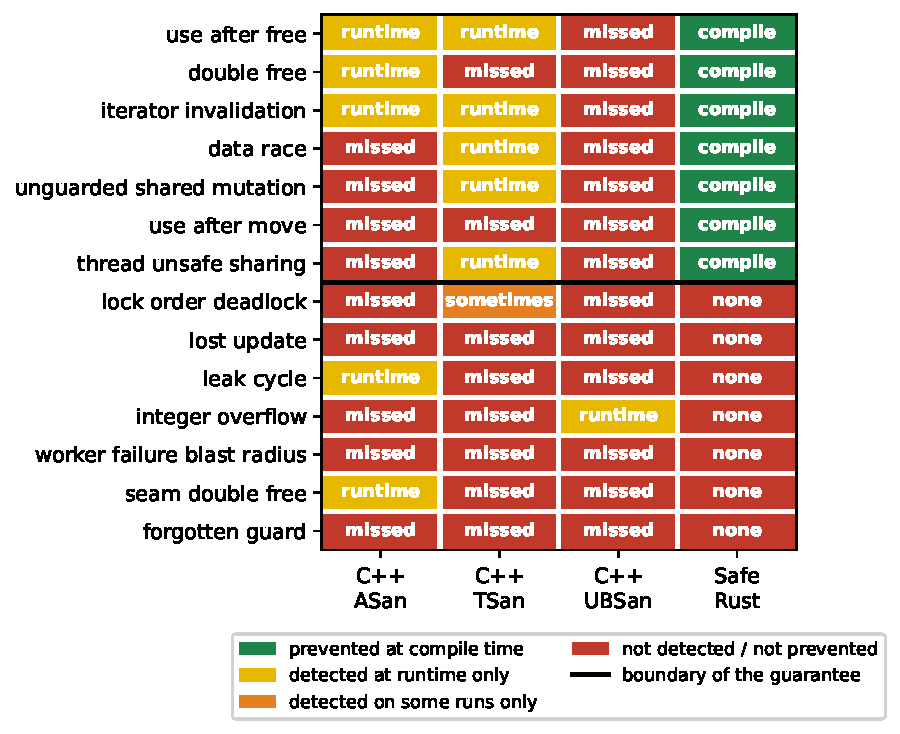
\includegraphics[width=0.9\linewidth]{figures/fig_taxonomy.pdf}
\caption{Defect-class outcome matrix. Green cells are defects prevented at compile time
(safe Rust); amber cells are defects that compile in C++ but are caught at runtime by the
given sanitiser; red cells are defects the sanitiser does not detect. Generated from the
fault-injection runner logs.\label{fig:taxonomy}}
\end{figure}

\subsection{Migration (RQ4)}
Incremental adoption is assessed with a working prototype that models the realistic
direction of migration: an existing C++ host keeps a Rust component behind a C ABI. The Rust
service is exposed through a thin \texttt{extern "C"} seam in a \emph{separate} crate that
depends on the unmodified core library, so adopting the component requires no changes to the
component itself. The C++ host sees only an opaque handle and a set of plain-C entry points
(a hand-written header, no generated bindings), and drives the full UE lifecycle across the
boundary; the error model is transported faithfully (for example, a duplicate connection
setup returns \texttt{InvalidState} through the seam).

\begin{figure}
\centering
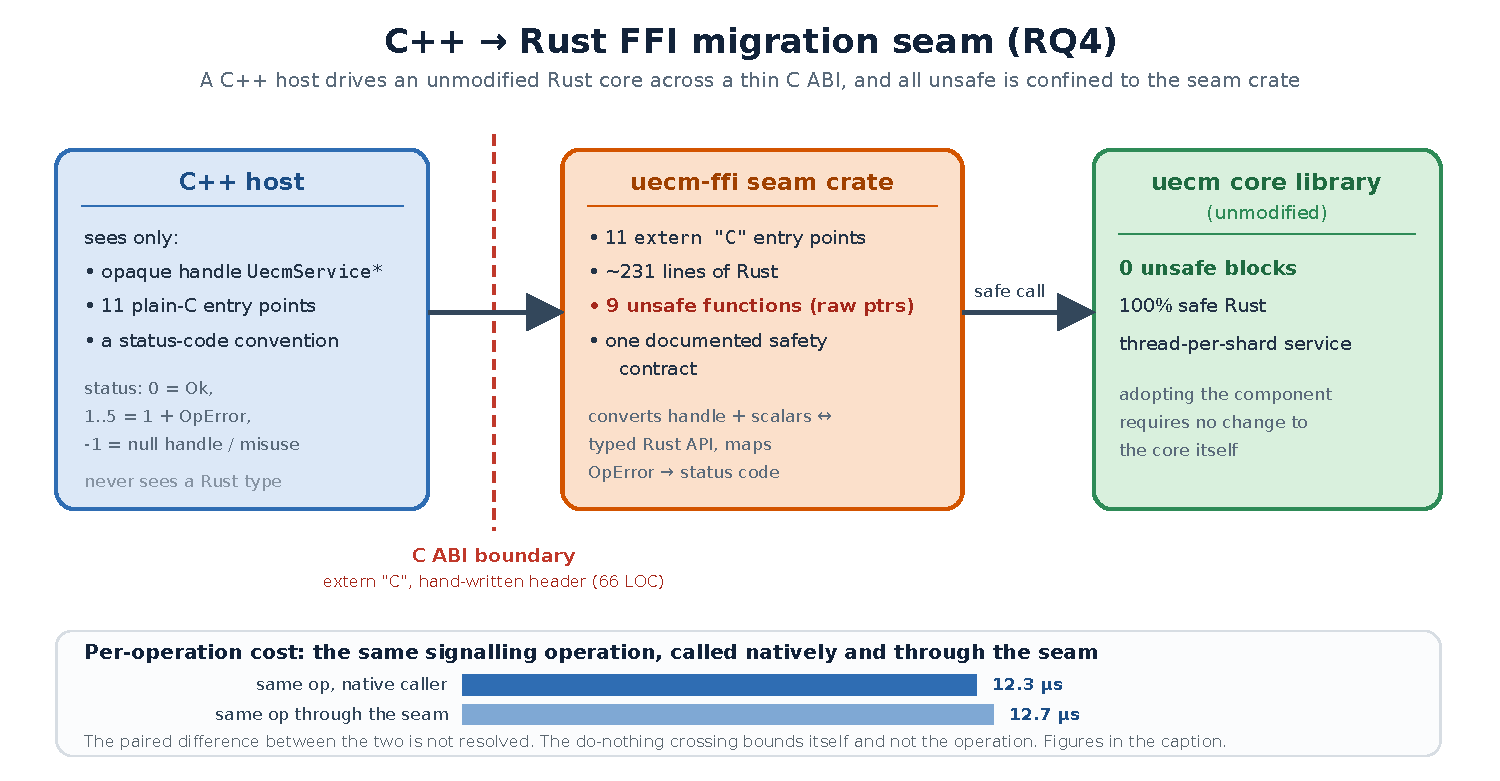
\includegraphics[width=\linewidth]{diagrams/pdf/07_ffi_seam.pdf}
\caption{The C++-to-Rust FFI migration seam. The C++ host sees only an opaque handle, twelve
plain-C entry points, and a status-code convention; a thin \texttt{extern "C"} seam crate
concentrates all of the raw-pointer \texttt{unsafe} (twelve sites) and calls the unmodified Rust
core, which remains free of \texttt{unsafe}. The do-nothing crossing costs a fraction of a
nanosecond, roughly five orders of magnitude below the cost of a signaling
operation.\label{fig:ffiseam}}
\end{figure}

The prototype yields concrete interop-cost figures, summarised in Table~\ref{tab:ffi}. The
seam is small, twelve C-ABI entry points in roughly $230$ lines of Rust plus a $66$-line C
header, with no third-party FFI dependency. The safety boundary is clean: the core library
remains free of \texttt{unsafe}, and the raw-pointer handling the C ABI requires is confined
to the seam crate (its twelve \texttt{unsafe} sites) under a single documented safety
contract, so the C++ side never sees a Rust type. Crucially, the boundary imposes no
measurable per-call tax: as Figure~\ref{fig:ffi-cost} shows, a do-nothing crossing measures
well under one nanosecond per call (an ordinary indirect call), roughly five orders of
magnitude below the end-to-end cost of a signaling operation, which is dominated by the
service's cross-thread submit-and-complete round-trip that a native (non-FFI) caller pays
identically. The main engineering effort is therefore in \emph{designing} a C-compatible API
surface, an opaque handle, scalar-typed operations, and a status convention, rather than in
any runtime overhead. The reverse direction (Rust calling into C++) is symmetric but requires
a C-ABI wrapper on the C++ side and re-introduces \texttt{unsafe} at the Rust caller. The
prototype and its measurements are published with the thesis, and inform the migration
guidelines of Chapter~\ref{chapter:discussion}.

\begin{table}
\centering
\caption{FFI migration prototype: seam size, safety boundary, and per-call interop cost
(C++ host calling the Rust component across a C ABI, \texttt{-O2}). The core library is
unmodified and \texttt{unsafe}-free; all interop is confined to the seam crate.\label{tab:ffi}}
\begin{tabular}{l r}
\hline\hline
Metric & Value \\
\hline
C-ABI entry points & 12 \\
Seam size (Rust \texttt{lib.rs}) & 231 LOC \\
Hand-written C header & 66 LOC \\
\texttt{unsafe} in core library & 0 \\
\texttt{unsafe} in FFI seam & 12 \\
Raw FFI crossing & 2.54 ns/call \\
Signaling op, native caller & 12.3 \textmu s/call \\
Signaling op, through the seam & 12.7 \textmu s/call \\
Seam cost per operation (paired) & $+192$ ns $[-954, +1341]$ \\
\quad as a fraction of the operation & $+10.91\%$ at the upper bound
\\
\hline
\end{tabular}
\end{table}

\begin{figure}
\centering
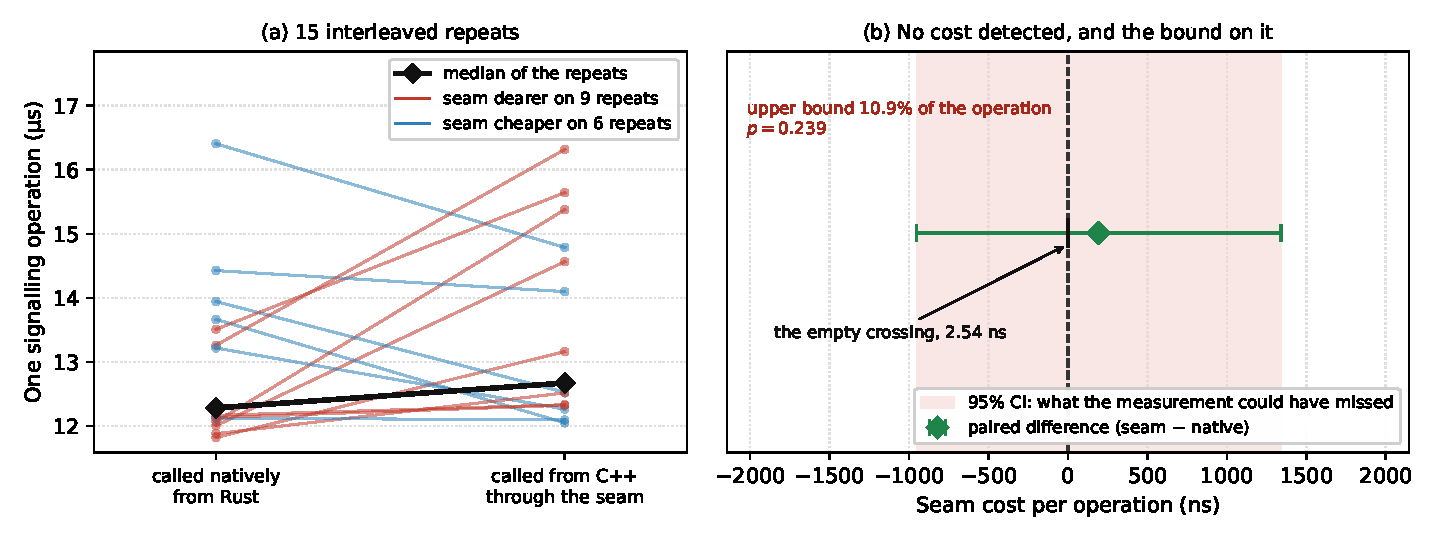
\includegraphics[width=0.78\linewidth]{figures/fig_ffi_cost.pdf}
\caption{Per-call cost of crossing the C ABI (a do-nothing \texttt{extern "C"} call) versus
the end-to-end cost of one signaling operation through the seam. Log-scaled $y$-axis: the FFI
crossing is negligible next to the service's cross-thread round-trip.\label{fig:ffi-cost}}
\end{figure}

\chapter{Discussion\label{chapter:discussion}}

\section{Summary of findings}
Table~\ref{tab:findings} collects the headline finding for each research question together
with the strength of the current evidence. The safety and migration results (RQ2, RQ4) are
final, because they do not depend on the measurement environment; the performance and resource
results (RQ1, RQ3) are reported from the development-environment campaign and are expected to
hold on the bare-metal testbed, but are labelled preliminary until that campaign is run.

\begin{table}
\centering
\caption{Summary of findings per research question and the current strength of evidence.
\label{tab:findings}}
\renewcommand{\arraystretch}{1.25}
\begin{tabular}{@{}p{0.06\linewidth} p{0.62\linewidth} p{0.22\linewidth}@{}}
\hline\hline
RQ & Headline finding & Evidence status \\
\hline
RQ1 & Rust and C++ track each other closely up to saturation (medians within a few
microseconds, p99 within $\sim$20\%); differences appear only in the far tail, where the
allocator matters as much as the language. & Preliminary (WSL2) \\
RQ2 & Every one of the five injected C++ defect classes is prevented at compile time in safe
Rust; in C++ each compiles and is caught, if at all, only at runtime, and no single sanitiser
covers the whole catalogue. & Final \\
RQ3 & Peak RSS and CPU utilisation are comparable across languages; \texttt{jemalloc} trades a
few MiB of RSS for a shorter tail. & Preliminary (WSL2) \\
RQ4 & The FFI seam is small, keeps the core \texttt{unsafe}-free, and imposes no measurable
per-call tax (sub-nanosecond crossing vs.\ a $\sim$$80\,\mu$s operation); the real cost is
API design, not run-time overhead. & Final \\
\hline
\end{tabular}
\end{table}

\section{Discussion on the research questions}
\paragraph{RQ1 (predictability).} The preliminary sweep supports the hypothesis that the two
languages are, for this workload, performance-equivalent in the region that matters
operationally: below saturation their median and p99 latencies are indistinguishable within
run-to-run noise, and the tail only separates once the blocking-backpressure design pushes the
system into overload. This is consistent with the wider evidence that Rust's safety checks are
largely absorbed by modern CPUs~\cite{emmerich2019drivers,balasubramanian2017rust}, and it
shifts the practical question from ``is Rust fast enough?'' to ``how does each language behave
at the overload cliff?'', a question the bare-metal campaign is designed to answer with the
frequency and scheduling controls WSL2 cannot provide.

\paragraph{RQ2 (safety).} The result is unambiguous and does not depend on the environment:
the borrow checker rejects all five defect classes at compile time, so they cannot be written
in safe Rust, whereas in C++ each is valid code detected only at runtime and only under the
right sanitiser and a test that exercises the buggy path. This is a qualitative,
kind-of-guarantee difference rather than a quantitative one, and it aligns with the CVE
evidence that Rust memory-safety bugs invariably involve \texttt{unsafe}~\cite{xu2021rustcve}
and with the caution that unsafety can still propagate through
dependencies~\cite{evans2020rust}, which is why keeping the core \texttt{unsafe}-free (as
done here) matters.

\paragraph{RQ3 (overhead).} No systematic memory or CPU penalty for Rust's safety model is
observed at the tested loads; resource use is dominated by the shared design rather than by the
language, and allocator choice is a larger lever than language choice. As with RQ1, the
absolute numbers await the testbed, but the \emph{relative} picture (no language-level penalty)
is expected to be robust.

\paragraph{RQ4 (migration).} The prototype shows that incremental adoption is technically
cheap: a C++ host can call an unmodified Rust core across a thin C-ABI seam with a
sub-nanosecond per-call cost, confining all \texttt{unsafe} to the seam. The dominant cost is
therefore human, not machine: designing a C-compatible surface and, per adoption
studies~\cite{fulton2021adopting}, climbing Rust's learning curve. This reframes migration
risk as an organisational rather than a performance concern.

\section{Related work}
Prior Rust-versus-C/C++ comparisons focus on general-purpose performance and
energy~\cite{pereira2017energy}, and cross-language benchmark surveys report that Rust matches
C and C++ on performance while adding safety~\cite{bugden2022rust}. Formal and empirical work establishes the soundness of
Rust's safe fragment and the disciplined use of \texttt{unsafe}: RustBelt provides
machine-checked foundations for the safety claims~\cite{jung2018rustbelt,jung2021safe} and the
Stacked Borrows model formalises the aliasing rules that \texttt{unsafe} code must
respect~\cite{jung2020stacked}, while
empirical studies of real-world code and of all known memory-safety CVEs show that
\texttt{unsafe} is used sparingly and that memory-safety defects invariably trace back to it
~\cite{astrauskas2020unsafe,qin2020rust,xu2021rustcve}; a complementary study cautions that
unsafety nonetheless propagates through dependency call chains, so most libraries cannot be
fully statically checked~\cite{evans2020rust}. Industry and government reports motivate memory
safety from a security standpoint and now call for migration to memory-safe
languages~\cite{msrc2019memory,google2022android,cisa2023memorysafe,oncd2024building,google2024securebydesign};
the long-standing difficulty of containing memory-corruption attacks in C/C++ with runtime
mitigations alone is the security backdrop to this shift~\cite{szekeres2013sok}. On the
performance side, systems-oriented studies argue that Rust delivers safety at essentially zero
runtime cost and is viable in demanding low-level domains: Rust enforces safety without
garbage-collection overhead and enables efficiency techniques impractical in
C~\cite{balasubramanian2017rust}, embedded/real-time systems such as a Rust hypervisor have
been shown to gain memory safety without sacrificing performance~\cite{mo2023rustshyper},
production cloud infrastructure such as AWS Firecracker is built in Rust~\cite{agache2020firecracker}, and
in the networking domain an idiomatic Rust user-space driver runs within a few percent of its
C reference~\cite{emmerich2019drivers}. The predictability angle draws on the tail-latency and
microsecond-scale latency literature~\cite{dean2013tail,barroso2017microseconds,li2014tales}, the RAN
context on the O-RAN disaggregation trend~\cite{polese2023oran}, and the adoption angle on
qualitative studies reporting that the main barrier to Rust is its learning curve rather than
run-time cost~\cite{fulton2021adopting}. Measurement methodology follows established guidance
on statistically rigorous, repeat-based performance evaluation~\cite{georges2007rigorous}, and
the fault-injection study follows standard software-fault-injection practice~\cite{natella2016fault}.
This thesis complements that body of work by targeting tail-latency predictability and
migration cost for a telecom control-plane workload under overload, an application domain and
operating regime the prior comparisons do not cover.

Not all of this evidence points the same way, and the thesis takes the qualifying findings
seriously rather than citing only the favourable ones. Even the positive networking result
records a real cost: the idiomatic Rust driver issues substantially more instructions per
packet than its C reference and is measurably slower in absolute terms, its safety checks
being absorbed by out-of-order execution rather than being literally
free~\cite{emmerich2019drivers}; the ``zero-cost'' framing~\cite{balasubramanian2017rust} is
therefore better read as workload-dependent than as universal, which is precisely why tail
behaviour must be measured on the target workload rather than assumed. The safety story is
likewise not absolute: empirical studies of real-world Rust find that memory- and
thread-safety bugs still occur in practice, with blocking bugs and misused synchronisation
among them~\cite{qin2020rust}, and that a substantial fraction of the ecosystem cannot be
fully statically checked because \texttt{unsafe} propagates through dependency
chains~\cite{evans2020rust}. These qualifications do not overturn the case for Rust, but they
motivate two of the thesis's design choices: measuring predictability and defect prevention
directly on the subsystem instead of importing general-purpose, average-case conclusions, and
keeping the safety-critical core \texttt{unsafe}-free so that the dependency-propagation
caveat does not apply to it.

\section{Threats to validity and mitigations}
The central threat is implementation bias between the two versions; it is mitigated by the
frozen shared specification (Section~\ref{sec:fairness}), identical algorithms, data
structures, and concurrency model, identical allocator and build optimisation, and
independent functional parity testing (Section~\ref{sec:parity}). Reliability of the quantitative results rests on
repeated runs with reported confidence intervals and histogram-based latency capture that
avoids coordinated-omission bias~\cite{tene_hdrhistogram}. Remaining threats include
single-author skill asymmetry, the use of a synthetic workload rather than captured
production traces, a single simplified subsystem (limiting generalisation to PHY/L2 or other
hardware), and the question of whether the chosen metrics faithfully capture predictability
and error-proneness; qualitative findings are reported as such.

\chapter{Conclusion and Future Work\label{chapter:conclusions}}

This thesis compared modern C++ and Rust on a UE Context Management service modeled on a real
Nokia gNB-CU-CP component, along four dimensions: tail-latency predictability, compile-time
defect prevention, safety-model overhead, and incremental-adoption cost. Built against a single
frozen specification and driven through identical code paths, the two implementations let
language effects be isolated from design and skill differences.

Three conclusions follow from the evidence. First, on safety the difference is one of
\emph{kind}: safe Rust rejects all five injected defect classes at compile time, turning a class
of runtime hazards that C++ can only hope to catch with sanitiser-instrumented tests into
errors that cannot be written at all. Second, on migration the cost is dominated by API design
and the learning curve rather than by any run-time tax: an unmodified Rust core can be driven
from C++ across a thin, \texttt{unsafe}-isolated seam at sub-nanosecond per-call cost. Third, on
performance the preliminary evidence is that the two languages are equivalent in the
operationally relevant region below saturation, with differences confined to the far tail;
confirming this on a bare-metal testbed is the single most important remaining step, and the
published scripts regenerate every figure and table once that data is captured.

Several directions extend the work: replaying captured (anonymised) production traces instead
of a synthetic workload; scaling the comparison to additional control-plane subsystems or to
the data-heavy L2/PHY path; evaluating Rust async runtimes against the thread-per-shard model
used here; and a longer-term migration case study that tracks defect density and review effort
as Rust is adopted incrementally in a production RAN codebase.

% STEP 5:
% Uncomment the following lines and set your .bib file and desired bibliography style
% to make a bibliography with BibTeX.
% Alternatively you can use the thebibliography environment if you want to add all
% references by hand.

\cleardoublepage %fixes the position of bibliography in bookmarks
\phantomsection

\addcontentsline{toc}{chapter}{\bibname} % This lines adds the bibliography to the ToC
\bibliographystyle{abbrv} % numbering alphabetic order
\bibliography{bibliography}

\begin{appendices}
\myappendixtitle

\chapter{Fault-injection example\label{appendix:code}}
As an illustration of the fault-injection study (Chapter~\ref{chapter:eval}, RQ2), the
use-after-free defect is shown in both languages. In C++ the alias into the context map
survives the \texttt{erase} that frees it, so the following program compiles cleanly and is
flagged only at runtime by AddressSanitizer:

\begin{verbatim}
std::unordered_map<unsigned long, UeContext> ctxs;
ctxs[1001] = UeContext{1001, 0};
UeContext* p = &ctxs.at(1001);  // alias into the container
ctxs.erase(1001);               // frees the node that p refers to
p->messages_handled += 1;       // use-after-free
\end{verbatim}

The analogous safe-Rust program does not compile: the borrow checker forbids mutating the map
(\texttt{remove}) while the reference \texttt{p} into it is still live, so the defect cannot be
written in the first place (error \texttt{E0499}):

\begin{verbatim}
let mut ctxs: HashMap<u64, UeContext> = HashMap::new();
ctxs.insert(1001, UeContext { messages_handled: 0 });
let p = ctxs.get_mut(&1001).unwrap(); // mutable borrow starts
ctxs.remove(&1001);                   // borrow while p live -> rejected
p.messages_handled += 1;              // p used after the remove
\end{verbatim}

\end{appendices}

\end{document}
